\documentclass[10pt]{book}

\usepackage[sectionbib,authoryear,round]{natbib}
\usepackage{array,epsfig,fancyhdr,rotating}
\usepackage{amsmath,amssymb,amsfonts,amsthm,graphicx,booktabs,multirow,placeins}
\allowdisplaybreaks[1]
\usepackage{sectsty,secdot}
\usepackage{xr-hyper}
\usepackage[hidelinks]{hyperref}
\renewcommand{\bibsection}{\section*{References}}
\usepackage{etoolbox}
\AtBeginDocument{\apptocmd{\thebibliography}{\interlinepenalty=10000\clubpenalty=10000\widowpenalty=10000}{}{}}
\sectionfont{\fontsize{12}{14pt plus.8pt minus .6pt}\selectfont}
\subsectionfont{\fontsize{12}{14pt plus.8pt minus .6pt}\selectfont}
\textwidth=31.9pc
\textheight=46.5pc
\oddsidemargin=1pc
\evensidemargin=1pc
\headsep=15pt
\topmargin=.6cm
\parindent=1.7pc
\parskip=0pt
\emergencystretch=1em
\clubpenalty=10000
\widowpenalty=10000
\brokenpenalty=10000
\setcounter{page}{1}
\pagestyle{fancy}
\renewcommand{\sectionmark}[1]{}
\renewcommand{\subsectionmark}[1]{}
\lhead[\footnotesize\thepage\fancyplain{}\leftmark]{}
\chead[]{}
\rhead[]{\fancyplain{}\rightmark\footnotesize\thepage}
\cfoot{}
\fancypagestyle{firstpage}{\fancyhf{}\fancyhead[L]{\footnotesize\rm Statistica Sinica: Supplement}\fancyhead[R]{\footnotesize\thepage}}
\newtheorem{theorem}{Theorem}
\newtheorem{lemma}{Lemma}
\newtheorem{corollary}{Corollary}
\newtheorem{proposition}{Proposition}
\newtheorem{assumption}{Assumption}
\newtheorem{step}{Step}
\newtheorem{setting}{Setting}
\newtheorem{definition}{Definition}
\newtheorem{example}{Example}
\newtheorem{remark}{Remark}

\newcommand{\ba}{{\mathbf a}}
\newcommand{\bb}{{\mathbf b}}
\newcommand{\be}{{\mathbf e}}
\newcommand{\bh}{{\mathbf h}}
\newcommand{\br}{{\mathbf r}}
\newcommand{\bu}{{\mathbf u}}
\newcommand{\bv}{{\mathbf v}}
\newcommand{\bx}{{\mathbf x}}
\newcommand{\bA}{{\mathbf A}}
\newcommand{\bB}{{\mathbf B}}
\newcommand{\bC}{{\mathbf C}}
\newcommand{\bD}{{\mathbf D}}
\newcommand{\bE}{{\mathbf E}}
\newcommand{\bG}{{\mathbf G}}
\newcommand{\bH}{{\mathbf h}}
\newcommand{\bI}{{\mathbf I}}
\newcommand{\bK}{{\mathbf K}}
\newcommand{\bL}{{\mathbf L}}
\newcommand{\bM}{{\mathbf M}}
\newcommand{\bQ}{{\mathbf Q}}
\newcommand{\bR}{{\mathbf R}}
\newcommand{\bS}{{\mathbf S}}
\newcommand{\bT}{{\mathbf T}}
\newcommand{\bU}{{\mathbf U}}
\newcommand{\bV}{{\mathbf V}}
\newcommand{\bW}{{\mathbf W}}
\newcommand{\bX}{{\mathbf X}}
\newcommand{\bY}{{\mathbf Y}}
\newcommand{\bZ}{{\mathbf Z}}
\newcommand{\bbeta}  {\boldsymbol{\beta}}
\newcommand{\btheta}  {\boldsymbol{\theta}}
\newcommand{\bmu} {\boldsymbol{{\mathbf \mu}}}
\newcommand{\bpsi} {\boldsymbol{{\mathbf \psi}}}
\newcommand{\bxi} {\boldsymbol{{\mathbf \xi}}}
\newcommand{\bGamma} {\boldsymbol{\Gamma}}
\newcommand{\bSigma} {\boldsymbol{\Sigma}}
\newcommand{\bPsi} {\boldsymbol{\Psi}}
\newcommand{\bPhi} {\boldsymbol{\Phi}}
\newcommand{\bXi} {\boldsymbol{\Xi}}
\newcommand{\bOmega} {\boldsymbol{\Omega}}
\newcommand{\bDelta} {\boldsymbol{\Delta}}
\newcommand{\real}{\mathbb{R}}
\newcommand{\expect}{\mathbb{E}}
\newcommand{\prob}{\mathbb{P}}
\newcommand{\Var}{\textrm{Var}}
\newcommand{\Cov}{\textrm{Cov}}
\newcommand{\diag}{\textrm{diag}}

\newcommand{\trans}{{\scriptscriptstyle\mathsf{T}}}
\newcommand{\wh}{\widehat}
\newcommand{\wt}{\widetilde}
\newcommand{\bone}{{\mathbf 1}}
\newcommand{\supp}{{\mathrm supp}}



\numberwithin{equation}{section}
\newcommand{\bodyfont}{\fontsize{12}{14pt plus.8pt minus .6pt}\selectfont}
\newcommand{\referencefont}{\bibhang=1.7pc\bibsep=2pt\fontsize{9}{14pt plus.8pt minus .6pt}\selectfont}
\externaldocument[][nocite]{fscb-draft}

\begin{document}
\renewcommand{\baselinestretch}{2}
\bodyfont
\markboth{\hfill{\footnotesize\rm HAOZHEN SHU, ZHENHUA LIN AND YINAN LIN}\hfill}
{\hfill{\footnotesize\rm BANDS FOR FUNCTIONAL REGRESSION}\hfill}
\thispagestyle{firstpage}
$\ $\par\vspace{0.8pc}
\centerline{\large\bf SIMULTANEOUS CONFIDENCE BANDS FOR}
\vspace{2pt}
\centerline{\large\bf FUNCTIONAL VARYING-COEFFICIENT MODELS}
\vspace{.4cm}
\centerline{Haozhen Shu$^1$, Zhenhua Lin$^2$ and Yinan Lin$^3$}
\vspace{.4cm}
\centerline{\it $^1$National Institute of Education,}
\centerline{\it Nanyang Technological University,}
\centerline{\it $^2$National University of Singapore and}
\centerline{\it $^3$Chongqing Normal University}
\vspace{.55cm}

\raggedbottom
\centerline{\bf Supplementary Material}
\vspace{.55cm}
\fontsize{9}{11.5pt plus.8pt minus.6pt}\selectfont
This supplement uses the notation of the main article. Sections S1--S2 prove the main results under the assumptions stated in the main article. Section S3 discusses sampling frequency, dimension, bandwidth, and implementation. Section S4 extends the analysis to high-dimensional functional means. Section S5 reports computational details and additional results.
\par\bodyfont
\setcounter{section}{0}
\def\thesection{S\arabic{section}}
\numberwithin{equation}{section}
\numberwithin{lemma}{section}
\numberwithin{proposition}{section}
\numberwithin{corollary}{section}
\numberwithin{theorem}{section}
\renewcommand{\thetable}{S\arabic{table}}
\renewcommand{\thefigure}{S\arabic{figure}}
\section{Linearization and covariance bounds}
\label{app:hd-linear-covariance}

In the proofs, we use $1+F_i$ when an auxiliary envelope bounded below
by one is convenient. Since $K_n\ge1$,
$\|1+F_i\|_{L^q}\le1+K_n\le2K_n$, so this does not change any rate.

We use Assumptions~\ref{ass:core}--\ref{ass:covariance} from the main
article. Constants are uniform in $n,p,h$ and the observation counts;
$r$ and $q$ are fixed, and $s=r+1$.
Write $P=(r+1)p$ and use $\|\cdot\|_{\max}$ for the largest absolute
entry of a vector or matrix at one time point. Estimation, residuals,
and inference all use $\mathcal T=[0,1]$. All other notation is as in
Sections~\ref{sec:method} and~\ref{sec:theory}.

We use the scales in \eqref{eq:basic-rates},
\eqref{eq:gaussian-rate}, and \eqref{eq:bootstrap-covariance-scales},
and the local basis and block selector from Section~\ref{sec:method}.
Set
\[
\begin{split}
\bS_i(t)&=m_i^{-1}\sum_jK_h(T_{ij}-t)
\bpsi_{ij}(t)\bpsi_{ij}(t)^\trans,\qquad
\widehat{\bD}_h=n^{-1}\sum_i\bS_i,\\
\bu_i(t)&=m_i^{-1}\sum_jK_h(T_{ij}-t)
\bpsi_{ij}(t)\varepsilon_i(T_{ij}),\qquad
\bar\bu=n^{-1}\sum_i\bu_i,\\
\bD_h(t)&=\expect\{\widehat{\bD}_h(t)\},\qquad
\bPsi_i(t)=\bL\bD_h(t)^{-1}\bu_i(t).
\end{split}
\]

\subsection{Population design and uniform concentration}

\begin{lemma}[Population design]\label{lem:hd-population}
Under Assumptions~\ref{ass:core}, \ref{ass:design}, and
\ref{ass:kernel}, uniformly on $\mathcal T$,
\[
c_D\bI_P\preceq\bD_h(t)\preceq C_D\bI_P,
\qquad
\|\bD_h(t)-\bD_h(u)\|_{\mathrm{op}}
\le Ch^{-1}|t-u|.
\]
Define the kernel-window moment matrix by
\[
\begin{gathered}
I_{t,h}=[-1,1]\cap[-t/h,(1-t)/h],\\
\bGamma_r(t,h)=\int_{I_{t,h}}
\btheta_r(z)\btheta_r(z)^\trans K(z)\,dz.
\end{gathered}
\]
Then, uniformly for $t\in\mathcal T$,
\[
\bD_h(t)=\bGamma_r(t,h)\otimes\{f(t)\bOmega(t)\}
+O_{\mathrm{op}}(h).
\]
\end{lemma}

\begin{proof}
The exact formula is
\[
\bD_h(t)=\int_{I_{t,h}}\btheta_r(z)\btheta_r(z)^\trans K(z)
\otimes\{f(t+hz)\bOmega(t+hz)\}\,dz.
\]
For $h\le1/2$, this interval contains either $[0,1]$ or $[-1,0]$.
Continuity, symmetry, nonnegativity, and unit integral imply that $K$
is positive on a nonempty interval in $(0,1)$ and on its reflection.
The polynomial Gram matrix on either half is positive definite:
a nonzero polynomial cannot vanish on such an interval.  Its dimension
$r+1$ is fixed.  The eigenvalue bounds for $f\bOmega$ therefore give
the asserted uniform lower bound; the upper bound
follows from boundedness of the basis and the kernel.
The $L^1$ increment, between evaluation points $t$ and $s$, of each
scalar kernel $u\mapsto K_h(u-t)((u-t)/h)^a$, $0\le a\le2r$,
is at most $Ch^{-1}|t-s|$.
Integrating against the operator-bounded $f\bOmega$ proves the
increment bound. Operator-norm Lipschitz continuity of $f\bOmega$
on $\mathcal T$ gives the stated expansion with $\bGamma_r(t,h)$,
uniformly in $t$.  The inverse matrices have
the same uniform operator bound and an $O(h^{-1})$ Lipschitz constant
by the resolvent identity.
\end{proof}

For the Taylor remainder, put
\[
\begin{aligned}
\br(t,u)&=\bbeta(u)-\sum_{a=0}^r
\frac{\bbeta^{(a)}(t)}{a!}(u-t)^a,
\\
\ba_i(t)&=m_i^{-1}\sum_jK_h(T_{ij}-t)
\bpsi_{ij}(t)\bX_{ij}^\trans\br(t,T_{ij}),
\end{aligned}
\]
and $\ba_n=n^{-1}\sum_i\ba_i$. Each coordinate of $\br$ is bounded
by $Ch^s$ on the kernel support, so
$\|\br(t,u)\|_2\le C\sqrt p\,h^s$ there.

\begin{lemma}[Uniform first and second moments]
\label{lem:hd-concentration}
Under Assumptions~\ref{ass:core}--\ref{ass:moments}, define
\[
\begin{gathered}
\mathcal D_n=\sup_t\|\widehat{\bD}_h(t)-\bD_h(t)\|_{\mathrm{op}},\quad
\mathcal U_n=\|\bar\bu\|_{\infty,\mathcal T},\\
\mathcal A_n=\frac{\|\ba_n-\expect\{\ba_n\}\|_{2,\mathcal T}}
{\sqrt p\,h^s}.
\end{gathered}
\]
Then
\[
\expect(\mathcal D_n^2+\mathcal A_n^2)\le C\rho_n^2,
\qquad \expect(\mathcal U_n^2)\le C\delta_n^2.
\]
Moreover,
\[
\|\expect\{\ba_n\}\|_{2,\mathcal T}\le C\sqrt p\,h^s.
\]
\end{lemma}

\begin{proof}
We first obtain a matrix variance bound from the existing coordinate
moments and the upper eigenvalue bound for $\bOmega$. For every
$\|\bv\|_2=1$, Minkowski's inequality gives
$\|\bv^\trans\bX(u)\|_{L^{2q}}\le C\sqrt p$, whereas
$\|\bv^\trans\bX(u)\|_{L^2}\le C$. Interpolation and H\"older's
inequality therefore imply
\[
\begin{split}
\expect\{X_k(u)^2(\bv^\trans\bX(u))^2\}
&\le C\|\bv^\trans\bX(u)\|_{L^{2q/(q-1)}}^2
\le Cp^{1/(q-1)},\\
\left\|\expect\{\|\bX(u)\|_2^2\bX(u)\bX(u)^\trans\}
\right\|_{\mathrm{op}}&\le Cp^{q/(q-1)}.
\end{split}
\]
These bounds hold uniformly in $u$. The bounded, fixed-dimensional
local polynomial basis preserves them up to a constant.

Condition on a subject's trajectories and separate identical from
distinct observation indices in the second moments. Identical indices
contribute a kernel integral of order $h^{-1}$; distinct indices
contribute bounded double integrals. For the latter, the squared
conditional mean is bounded by the weighted integral of the squared
mark. Explicitly, for a nonnegative weight $w$ and self-adjoint
matrix $A(u)$,
\[
\left\{\int w(u)A(u)\,du\right\}^2
\preceq\left\{\int w(u)\,du\right\}
\int w(u)A(u)^2\,du.
\]
Apply this with $w(u)=K_h(u-t)f(u)$ and the matrix mark
$\btheta_r\btheta_r^\trans\otimes\bX_i(u)\bX_i(u)^\trans$;
the vector version applies to the Taylor mark.
The matrix moment bound and
$\|\br(t,u)\|_2\le C\sqrt p\,h^s$ thus give
\[
\begin{gathered}
\left\|\expect\{(\bS_i(t)-\expect\bS_i(t))^2\}
\right\|_{\mathrm{op}}
\le Cp^{q/(q-1)}\{1+(m_i h)^{-1}\},\\
\frac{\expect\|\ba_i(t)-\expect\ba_i(t)\|_2^2}{p h^{2s}}
\le Cp^{q/(q-1)}\{1+(m_i h)^{-1}\}.
\end{gathered}
\]
The subject envelopes of $\bS_i$ in spectral norm and of
$\ba_i/(\sqrt p\,h^s)$ in Euclidean norm are at most
$Ch^{-1}\sup_u\|\bX_i(u)\|_2^2$. Minkowski's inequality gives
\[
\left\|\sup_u\|\bX_i(u)\|_2^2\right\|_{L^q}
\le\sum_{k=1}^p\left\|\sup_u|X_{ik}(u)|^2\right\|_{L^q}
\le Cp.
\]

Use a uniform grid $\chi_n$ of mesh at most
\[
\Delta_n=n^{-8}h^{10}(pK_n)^{-8},
\]
Then $\log(2P|\chi_n|)\le CL_n$.
For each subject, form a block diagonal matrix whose blocks are the
centered design matrices at all grid points. Its spectral norm is
the largest block norm, and the matrix variance parameter of the sum
is at most $Cnp^{q/(q-1)}v_n^2$. Its largest summand has $L^2$ norm
at most $Cpn^{1/q}/h$.
The second-moment inequality in Theorem~I of
\citet{tropp_expected_2016}, divided by $n$, yields
\[
\begin{aligned}
&\left[\expect\max_{t\text{ on grid}}
\|\widehat{\bD}_h(t)-\bD_h(t)\|_{\mathrm{op}}^2\right]^{1/2}\\
&\le C\left\{p^{q/(2q-2)}v_n\sqrt{L_n/n}
+\frac{pL_n}{n^{1-1/q}h}\right\}=C\rho_n.
\end{aligned}
\]
Apply the rectangular version of the same inequality to a block
diagonal matrix with column blocks
$\{\ba_i(t)-\expect\ba_i(t)\}/(\sqrt p\,h^s)$.
Both matrix variance parameters are bounded by the displayed vector
second moments. This proves the same grid bound for $\mathcal A_n$.

For the score, every coordinate has envelope $CF_i/h$ and second
moment at most $C\{1+(m_i h)^{-1}\}$. Applying Lemmas~E.1 and
E.2(ii) of \citet{chernozhukov_central_2017} simultaneously to the
score coordinates and grid points gives expected maximum at most
$C\delta_n$ and, above twice that expectation, the tail bound
\[
\exp(-cnx^2/v_n^2)+
\frac{Cn^{1-q}K_n^q}{h^q x^q},\qquad x>0.
\]
Integrating, with the polynomial term capped at one, gives the score
second moment bound because $q>2$.

The samplewise Lipschitz constants of the design in spectral norm
and of $\ba_i/(\sqrt p\,h^s)$ in Euclidean norm are at most
$CpF_i h^{-2}$; score coordinates have constants $CF_i h^{-2}$.
For the Taylor term, use
$|\partial_t r_k(t,u)|\le C|u-t|^r$ almost everywhere on the kernel
support; for $r=0$, use the Lipschitz property of $\beta_k$.
The compactly supported Lipschitz kernel gives the same increment
bound across the support boundary. Thus interpolation errors have
$L^2$ norm at most $CpK_n\Delta_n h^{-2}$, which is absorbed by the
respective rates.
Finally,
\[
\expect\{\ba_n(t)\}=\int K_h(u-t)
\{\btheta_r((u-t)/h)\otimes\bOmega(u)\}\br(t,u)f(u)\,du.
\]
The operator bound for $\bOmega$, the bounded basis, and
$\|\br(t,u)\|_2\le C\sqrt p\,h^s$ prove the last assertion.
\end{proof}

\begin{lemma}[Uniform linear representation]\label{lem:hd-linear}
Suppose Assumptions~\ref{ass:core}--\ref{ass:moments} hold and
$\rho_n\to0$. With probability tending to one,
$\widehat{\bD}_h$ is invertible throughout $\mathcal T$, and
\[
\widehat{\bbeta}(t)-\bbeta(t)
=n^{-1}\sum_i\bPsi_i(t)+\bR_n(t),\qquad t\in\mathcal T.
\]
Uniformly on this domain,
\[
\|\widehat{\bbeta}-\bbeta\|_2
=O_P\{\sqrt p(\delta_n+h^s)\},\qquad
\|\bR_n\|_{\max}
=O_P\{\sqrt p(\rho_n\delta_n+h^s)\}.
\]
More precisely, there is an event $\mathcal E_n$ with
$\prob(\mathcal E_n^c)\le C\rho_n^2$ such that, on this event,
\[
\begin{gathered}
\sup_t\|\widehat{\bD}_h(t)^{-1}\|_{\mathrm{op}}\le C,\qquad
\|\widehat{\bD}_h^{-1}-\bD_h^{-1}\|_{\mathrm{op},\mathcal T}
\le C\mathcal D_n,\\
\|\widehat{\bbeta}-\bbeta\|_{2,\mathcal T}
\le C\sqrt p(\mathcal U_n+h^s),\qquad
\|\bR_n\|_{\infty,\mathcal T}
\le C\sqrt p\,\mathcal D_n\mathcal U_n+C\sqrt p\,h^s.
\end{gathered}
\]
\end{lemma}

\begin{proof}
Let
\[
\mathcal E_n=\{\mathcal D_n\le c_D/2,\quad \mathcal A_n\le1\}.
\]
Lemma~\ref{lem:hd-concentration} and Markov's inequality give its
exceptional probability.  Weyl's inequality and the resolvent
identity give the two inverse bounds.  On $\mathcal E_n$,
\[
\|\ba_n\|_{2,\mathcal T}
\le C\sqrt p\,h^s+\sqrt p\,h^s\mathcal A_n
\le C\sqrt p\,h^s.
\]
The exact normal equation is
\[
\widehat{\bbeta}-\bbeta
=\bL\widehat{\bD}_h^{-1}(\bar\bu+\ba_n).
\]
Here the Taylor coefficients are stacked with their factors
$h^a/a!$, so their first block is exactly $\bbeta(t)$.
Since $\|\bar\bu\|_2\le\sqrt P\,\mathcal U_n$, the estimation
bound follows.  Subtracting $\bL\bD_h^{-1}\bar\bu$ yields
\[
\bR_n=\bL(\widehat{\bD}_h^{-1}-\bD_h^{-1})\bar\bu
+\bL\widehat{\bD}_h^{-1}\ba_n.
\]
Its first term is at most $C\sqrt p\,\mathcal D_n\mathcal U_n$ in
Euclidean norm, and hence in maximum norm.  The second is at most
$C\sqrt p\,h^s$ on $\mathcal E_n$. Lemma~\ref{lem:hd-concentration}
also gives
$\expect(\mathcal D_n\mathcal U_n)\le C\rho_n\delta_n$
by Cauchy--Schwarz. This proves all assertions and the quantitative
transfer bound used below.
\end{proof}

The preceding lemma proves Theorem~\ref{thm:linear}.

\subsection{Covariance and its sampling components}\label{app:covariance-proof}

\begin{lemma}[Covariance identity and variance order]
\label{lem:hd-covariance}
Under Assumptions~\ref{ass:core}--\ref{ass:covariance}, define
\[
\bA_h(t,u)=\bL\bD_h(t)^{-1}
\{\btheta_r((u-t)/h)\otimes\bI_p\}K_h(u-t).
\]
Then the covariance of $n^{-1/2}\sum_i\bPsi_i$ is
\[
\begin{split}
\bV_n(s,t)&=\kappa_{1,n}\bV_{h,d}(s,t)
+(1-\kappa_{1,n})\bV_{h,o}(s,t),\\
\bV_{h,d}(s,t)&=\int\bA_h(s,u)\bC(u,u)\bA_h(t,u)^\trans f(u)\,du,\\
\bV_{h,o}(s,t)&=\iint\bA_h(s,u)\bC(u,v)
\bA_h(t,v)^\trans f(u)f(v)\,du\,dv.
\end{split}
\]
Let $\be_0=(1,0,\ldots,0)^\trans$ and define
\[
\begin{gathered}
K_{r,t,h}(z)=\be_0^\trans\bGamma_r(t,h)^{-1}
\btheta_r(z)K(z)\mathbf1_{I_{t,h}}(z),\\
\nu_r(t,h)=\int K_{r,t,h}(z)^2\,dz.
\end{gathered}
\]
There are constants $0<c_\nu<C_\nu$ such that
$c_\nu\le\nu_r(t,h)\le C_\nu$ uniformly in $t,h$.
Uniformly on $\mathcal T$,
\[
\bV_n(t,t)=\left\{1-\kappa_{1,n}+
\frac{\kappa_{1,n}\nu_r(t,h)}{h f(t)}\right\}\bV_F(t)
+O_{\mathrm{op}}(hv_n^2).
\]
In particular, with $\tau_k^2(t)=[\bV_n(t,t)]_{kk}$,
\[
cv_n^2\le\tau_k^2(t)\le Cv_n^2\qquad(t\in\mathcal T, k\le p).
\]
\end{lemma}

\begin{proof}
Expand the two subject sums.  Identical observation indices have
score second moment $\bC(u,u)$; distinct indices have joint moment
$\bC(u,v)$ and independent times with density $f(u)f(v)$.
There are $m_i$ pairs of the first type and $m_i(m_i-1)$ of the
second.  Averaging the identity over subjects gives the result.
Both covariance components arise from the single functional error
process; their distinction concerns observation indices.

Lemma~\ref{lem:hd-population} and the operator inverse identity give,
uniformly for $t\in\mathcal T$ and $z\in I_{t,h}$,
\[
h\bA_h(t,t+hz)=\frac{K_{r,t,h}(z)}{f(t)}\bOmega(t)^{-1}
+O_{\mathrm{op}}(h).
\]
The moment identity
\[
\bGamma_r(t,h)\be_0=\int_{I_{t,h}}\btheta_r(z)K(z)\,dz
\]
implies $\int K_{r,t,h}=1$. The uniform inverse bound for
$\bGamma_r(t,h)$ gives $\nu_r(t,h)\le C$; Cauchy--Schwarz and
$|I_{t,h}|\le2$ give $\nu_r(t,h)\ge1/2$.
Changing variables in the two covariance integrals and using
operator-norm Lipschitz continuity gives, uniformly on $\mathcal T$,
\[
\begin{aligned}
\bV_{h,d}(t,t)&=\frac{\nu_r(t,h)}{hf(t)}\bV_F(t)
+O_{\mathrm{op}}(1),\\
\bV_{h,o}(t,t)&=\bV_F(t)+O_{\mathrm{op}}(h).
\end{aligned}
\]
The weighted error is at most $C(h+\kappa_{1,n})=Chv_n^2$.
The coordinate variances of $\bV_F$ are bounded above by the
operator bounds and below by assumption.  The scalar coefficient
in braces is comparable to $1+\kappa_{1,n}/h$, uniformly over
$0\le\kappa_{1,n}\le1$.  Absorbing the $O(hv_n^2)$ error proves
the variance bounds.
\end{proof}

Write
\[
\bT(t)=\operatorname{diag}(\tau_1^2(t),\ldots,\tau_p^2(t)),\qquad
\bM_i(t)=\bT(t)^{-1/2}\bPsi_i(t),
\]
and $\bQ_n(s,t)=n^{-1}\sum_i\expect\{\bM_i(s)\bM_i(t)^\trans\}$.
Thus each coordinate of the matching Gaussian process has variance
one, without any requirement that its full covariance be invertible.

\subsection{Oracle moments and empirical covariance}

\begin{lemma}[Subject moments and oracle covariance]
\label{lem:hd-oracle-covariance}
Under Assumptions~\ref{ass:core}--\ref{ass:covariance},
\[
\max_i\left\|\sup_{t\in\mathcal T}\|\bM_i(t)\|_\infty
\right\|_{L^q}\le\frac{C\sqrt p K_n}{hv_n},\qquad
\sup_{t,k}\frac1n\sum_i\expect\{|M_{ik}(t)|^4\}
\le Cp^2\Lambda_n.
\]
Moreover,
\[
\expect\{R_{Q,n}\}\le Ce_n,\qquad
R_{Q,n}=\left\|n^{-1}\sum_i\bM_i(s)\bM_i(t)^\trans
-\bQ_n(s,t)\right\|_{\infty,\mathcal T^2}.
\]
For
\[
J_{i,kl}(t)=m_i^{-1}\sum_jK_h(T_{ij}-t)|X_{ijk}X_{ijl}|,
\]
define
\[
\mathcal J_n=\max\left\{
\sup_{t,a}\frac1{nv_n^2}\sum_i u_{ia}(t)^2,
\sup_{t,k,l}\frac1{nv_n^2}\sum_iJ_{i,kl}(t)^2\right\}.
\]
There is a fixed $C_J$ for which
$\prob(\mathcal J_n>C_J)\le Ce_n$.
\end{lemma}

\begin{proof}
Every row of $\bL\bD_h^{-1}$ has uniformly bounded Euclidean norm,
so its sum of absolute entries is at most $C\sqrt p$.
Since every score coordinate is bounded by $CF_i/h$, this proves
the envelope bound.
For any scalar score entry, expanding its fourth moment into groups
with $d\in\{1,2,3,4\}$ distinct observation indices gives
\[
\expect\{|u_{ia}(t)|^4\}\le C\{1+(m_i h)^{-3}\}.
\]
Indeed, a time appearing $b$ times contributes
$\int|K_h(u-t)|^b f(u)\,du\le Ch^{1-b}$, mixed fourth mark
moments are uniformly bounded by H\"older's inequality, and the
group contains at most $Cm_i^d$ terms.  Its contribution is at most
$C(m_i h)^{d-4}$.  The same argument applies to $J_{i,kl}$.
Minkowski's inequality and the $C\sqrt p$ row-sum bound therefore
give a fourth moment at most $Cp^2\{1+(m_i h)^{-3}\}$ for each
$\Psi_{ik}$.  Divide by $\tau_k^4\asymp v_n^4$ and average.

For covariance products the average coordinate variance is at most
$Cp^2\Lambda_n$, by Cauchy--Schwarz and the last bound. Their
common envelope is $CpF_i^2/(h^2v_n^2)$, whose maximum over subjects
has $L^2$ norm at most
\[
\frac{Cp}{h^2v_n^2}
\left(\sum_i\expect\{F_i^q\}\right)^{2/q}
\le\frac{Cp n^{2/q}K_n^2}{h^2v_n^2}.
\]
Applying the same expectation maximal inequality to all signed
coordinate products and pairs of grid points gives
\[
\expect R_{Q,n}\le C\left\{p\sqrt{\Lambda_nL_n/n}
+\frac{pK_n^2L_n}{n^{1-2/q}h^2v_n^2}\right\}\le Ce_n.
\]

For completeness, interpolation here can also be controlled
uniformly in $p$.  The weights satisfy
\begin{align*}
\int\|\bA_h(t,u)-\bA_h(s,u)\|_{\mathrm{op}}^2 f(u)\,du
&\le Ch^{-3}|t-s|^2,\\
\int\|\bA_h(t,u)-\bA_h(s,u)\|_{\mathrm{op}}f(u)\,du
&\le Ch^{-1}|t-s|.
\end{align*}
These follow from the kernel increments and the $O(h^{-1})$
Lipschitz bound for $\bD_h^{-1}$.  The covariance identity and the
operator bound for $\bC$ imply
\[
\frac1n\sum_i\expect\{|\Psi_{ik}(t)-\Psi_{ik}(s)|^2\}
\le Cv_n^2h^{-2}|t-s|^2.
\]
The reverse triangle inequality in this $L^2$ norm gives
$|\tau_k(t)-\tau_k(s)|\le Cv_nh^{-1}|t-s|$.
Consequently, samplewise on $\mathcal T$,
\[
\sup_k|M_{ik}(t)-M_{ik}(s)|
\le\frac{C\sqrt p F_i}{v_nh^2}|t-s|.
\]
The expected covariance-product interpolation error is therefore
at most $CpK_n^2\Delta_n/(h^3v_n^2)$, which is absorbed by $e_n$,
since $e_n\ge p^{3/2}\delta_n\ge\sqrt{L_n/n}$.

Finally, each coordinate of $\bu_i/v_n$ and $J_{i,kl}/v_n$ has
average second moment bounded by a constant.  Their fourth moments
and product envelopes obey the same calculation with the row-sum
factor omitted (while keeping $L_n$ and $K_n$). Thus the expected
maximum fluctuation of their empirical squares is at most
\[
C\left\{\sqrt{\Lambda_nL_n/n}
+\frac{K_n^2L_n}{n^{1-2/q}h^2v_n^2}\right\}\le Ce_n.
\]
Markov's inequality at a fixed threshold above the population
second-moment bound proves the assertion about $\mathcal J_n$.
\end{proof}

\subsection{Fitted residuals and covariance control}

Let $\widehat\varepsilon_{ij}=Y_{ij}-\bX_{ij}^\trans
\widehat{\bbeta}(T_{ij})$, and define $\widehat\bu_i$ by replacing
$\varepsilon_i(T_{ij})$ in $\bu_i$ by this fitted residual.  Put
$\widehat{\bPsi}_i=\bL\widehat{\bD}_h^{-1}\widehat\bu_i$ and
\[
\widehat\sigma_k^2(t)=n^{-1}\sum_i\widehat\Psi_{ik}(t)^2,
\quad
\widehat{\bQ}_n(s,t)_{kl}=
\frac{n^{-1}\sum_i\widehat\Psi_{ik}(s)\widehat\Psi_{il}(t)}
{\widehat\sigma_k(s)\widehat\sigma_l(t)}.
\]
Let $\mathcal V_n$ be the event that $\widehat{\bD}_h$ is invertible
on $\mathcal T$ and all fitted coordinate variances are positive
on $\mathcal T$.  On this event define
\[
\vartheta_n=\sup_{t,k}\left|
\frac{\widehat\sigma_k(t)}{\tau_k(t)}-1\right|,
\qquad
\Delta_{Q,n}=\|\widehat{\bQ}_n-\bQ_n\|_{\infty,\mathcal T^2}.
\]
Set both quantities to $+\infty$ on $\mathcal V_n^c$.

\begin{lemma}[Quantitative feasible covariance]
\label{lem:hd-feasible-covariance}
Under Assumptions~\ref{ass:core}--\ref{ass:covariance}, if $e_n\to0$,
then, for all sufficiently large $n$ and $0<u\le1/2$,
\[
\prob\{\vartheta_n+\Delta_{Q,n}>u\}\le Ce_n/u.
\]
In particular, $\prob(\mathcal V_n^c)\le Ce_n$ and the discrepancies
are $O_P(e_n)$.  The fitted-score replacement obeys
\[
\sup_{t,k}\left[
\frac1n\sum_i
\left\{\frac{\widehat\Psi_{ik}(t)-\Psi_{ik}(t)}{\tau_k(t)}\right\}^2
\right]^{1/2}
=O_P\{p^{3/2}(\delta_n+h^s)\}.
\]
\end{lemma}

\begin{proof}
The condition $e_n\to0$ implies $p\delta_n\to0$ and hence
$\rho_n\to0$, so
Lemma~\ref{lem:hd-linear} applies.  Define
\[
\mathcal H_n=\mathcal E_n\cap\{R_{Q,n}\le1,
\ \mathcal J_n\le C_J\}.
\]
Its complement has probability at most $C(\rho_n^2+e_n)$.
Let $b_n^{\mathrm{fit}}=
\|\widehat{\bbeta}-\bbeta\|_{2,\mathcal T}$ and
$J_i^0(t)=\sum_kJ_{i,kk}(t)$.
Uniform empirical invertibility gives, on $\mathcal H_n$,
\[
\sup_{t,k}\sum_{a=1}^P|[\bL\widehat{\bD}_h(t)^{-1}]_{ka}|
\le\sqrt P\sup_t\|\bL\widehat{\bD}_h(t)^{-1}\|_{\mathrm{op}}
\le C\sqrt p.
\]
The residual identity and weighted Cauchy--Schwarz give, for a score
coordinate $a$ corresponding to predictor coordinate $k$,
\[
|\widehat u_{ia}(t)-u_{ia}(t)|
\le b_n^{\mathrm{fit}}\{J_{i,kk}(t)J_i^0(t)\}^{1/2}.
\]
Since $J_i^0=\sum_lJ_{i,ll}$, the definition of $\mathcal J_n$ implies
\[
\begin{gathered}
\sup_t\frac1{nv_n^2}\sum_i\|\bu_i(t)\|_2^2\le Cp,\\
\sup_{t,a}\frac1{nv_n^2}\sum_i
|\widehat u_{ia}(t)-u_{ia}(t)|^2
\le Cp(b_n^{\mathrm{fit}})^2.
\end{gathered}
\]
Indeed, each summand satisfies
\[
n^{-1}\sum_iJ_{i,kk}J_{i,ll}
\le \{n^{-1}\sum_iJ_{i,kk}^2\}^{1/2}
\{n^{-1}\sum_iJ_{i,ll}^2\}^{1/2}\le Cv_n^2.
\]
Use the exact decomposition
\[
\widehat{\bPsi}_i-\bPsi_i
=\bL(\widehat{\bD}_h^{-1}-\bD_h^{-1})\bu_i
+\bL\widehat{\bD}_h^{-1}(\widehat\bu_i-\bu_i).
\]
Applying the empirical $L^2$ norm to each coordinate and using
the empirical row-sum bound gives a fitted-score discrepancy at most
\[
\zeta_n=C\sqrt p\,\mathcal D_n
+Cp^{3/2}(\mathcal U_n+h^s),
\]
where we used $b_n^{\mathrm{fit}}\le C\sqrt p(\mathcal U_n+h^s)$.
Lemma~\ref{lem:hd-concentration} and $\rho_n\lesssim p\delta_n$ give
\[
\expect\zeta_n\le Cp^{3/2}(\delta_n+h^s),\qquad
\expect\zeta_n^2\le Cp^3(\delta_n+h^s)^2.
\]
No independence of fitted residuals and the fitting observations is
used in these inequalities.

Before dividing by fitted variances, write
\[
\mathcal W_n=\sup_{s,t,k,l}
\left|\frac{n^{-1}\sum_i
\widehat\Psi_{ik}(s)\widehat\Psi_{il}(t)}
{\tau_k(s)\tau_l(t)}-[\bQ_n(s,t)]_{kl}\right|.
\]
On $\mathcal H_n$, the empirical oracle coordinate second moments
are at most $2$, because $R_{Q,n}\le1$.  Expanding the difference
of products and applying Cauchy--Schwarz therefore gives
\[
\begin{aligned}
\mathcal W_n&\le R_{Q,n}+C\zeta_n+\zeta_n^2,\\
\expect\{\mathbf1_{\mathcal H_n}\mathcal W_n\}
&\le C\{e_n+p^3(\delta_n+h^s)^2\}\\
&\le Ce_n.
\end{aligned}
\]
The integrand is defined to be zero outside $\mathcal H_n$.
If $\mathcal W_n$ is smaller than a fixed constant, its diagonal
entries give positive fitted variances and fitted-to-oracle variance
ratios in $[1/2,3/2]$.  The square-root and inverse square-root maps
are Lipschitz on this interval.  Since $|[\bQ_n(s,t)]_{kl}|\le1$,
\[
\vartheta_n+\Delta_{Q,n}\le C\mathcal W_n
\]
on this event.  Consequently, for $0<u\le1/2$, Markov's inequality
and the exceptional-probability bound give
\[
\prob\{\vartheta_n+\Delta_{Q,n}>u\}
\le C(\rho_n^2+e_n)+Ce_n/u\le Ce_n/u.
\]
The last step uses $\rho_n^2\lesssim p^2\delta_n^2
\le p^3(\delta_n+h^s)^2\le e_n$ for all sufficiently large $n$.
This proves the tail bound, and the
fitted-score rate follows from its samplewise bound on
$\mathcal H_n$ and the vanishing exceptional probability.
\end{proof}

\section{Gaussian and bootstrap approximation}
\label{app:hd-approximation}\label{app:approximation-proofs}

Recall $L_n=\log(np/h)$, $s=r+1$, and let $\mathcal F_n$ denote the
sigma-field generated by the observations. All conditional probabilities
and expectations below condition on this sigma-field. Put
\[
 M_{ik}(t)=\Psi_{ik}(t)/\tau_k(t),\qquad
 Z_{n,k}(t)=n^{-1/2}\sum_i M_{ik}(t),
\]
and write
\[
Q_n(u,t)=n^{-1}\sum_i\expect\{M_i(u)M_i(t)^\trans\}.
\]
The matching Gaussian process $G_n$, its supremum $S_{G,n}$, the
statistics $T_n^\circ,T_n$, and the multiplier process and maximum
$G_n^*,S_n^*$ are those defined in Section~\ref{sec:theory}.

The preceding lemmas give the following inputs. The envelope $F_i$
in Assumption~\ref{ass:moments} satisfies $\|F_i\|_q\le CK_n$,
where $1\le K_n\le Cp^{1/q}$.
Lemma~\ref{lem:hd-covariance} gives $\tau_k(t)\asymp v_n$ uniformly.
The subject moment bounds imply
\begin{equation}
 \left\|\max_k\sup_t|M_{ik}(t)|\right\|_q\le CH_n,
 \qquad
 \max_k\sup_t\frac1n\sum_i\expect\{M_{ik}(t)^4\}\le CA_n,
 \label{eq:hd-standardized-inputs}
\end{equation}
where
\[
 H_n=\frac{\sqrt pK_n}{hv_n},\qquad
 A_n=p^2\Lambda_n,\qquad
 B_n=\max\{H_n,\sqrt{A_n}\}.
\]
The $\sqrt p$ row-sum bound for $\bL\bD_h^{-1}$ gives the score
envelope, and Minkowski's inequality gives the fourth-moment factor
$p^2$. These estimates use the general dimension bounds under the
stated assumptions. Since $h^2v_n^2\le h^2+h\le3/4$,
we have $H_n\ge1$, so a separate constant in the maximum defining
$B_n$ is unnecessary.

Use $\gamma_n,e_n$ from \eqref{eq:gaussian-rate} and
\eqref{eq:bootstrap-covariance-scales}, and write
\[
 r_{n,1}=\frac{\sqrt{np}\,\rho_n\delta_n}{v_n},\qquad
 r_{n,2}=\frac{\sqrt{np}\,h^s}{v_n}.
\]
The quantitative version of Lemma~\ref{lem:hd-linear}, including the
event controlling the centered Taylor score, gives, for every $u>0$,
\begin{equation}
 \prob\!\left\{\left\|
  \sqrt n\,\operatorname{diag}(\tau_k^{-1})(\wh\bbeta-\bbeta)
  -Z_n\right\|_{\infty,\mathcal T}>Cr_{n,2}+u\right\}
 \le C\rho_n^2+Cr_{n,1}/u.
 \label{eq:hd-transfer-input}
\end{equation}
In particular, the smoothing term in this bound is deterministic on an
event whose complement has probability at most $C\rho_n^2$;
an assertion in probability about the smoothing remainder alone would
not suffice for the coverage calculation below.

Let $\mathcal V_n$ be the event of uniform empirical design
invertibility and positive fitted variances. On its complement, extend
$T_n,S_n^*,G_n^*$ by zero and use empty bands. The statistic $T_n^\circ$
is extended by zero only when the empirical design fails to be uniformly
invertible. On $\mathcal V_n$, write
\[
 \vartheta_n=\max_k\sup_t
 \left|\frac{\widehat\sigma_k(t)}{\tau_k(t)}-1\right|,
 \qquad
 \Delta_{Q,n}=\|\widehat Q_n-Q_n\|_{\infty,\mathcal T^2},
\]
where
$\widehat Q_n(s,t)=n^{-1}\sum_i
 \widehat M_i(s)\widehat M_i(t)^\trans$ and
$\widehat M_{ik}=\widehat\Psi_{ik}/\widehat\sigma_k$.
Set both discrepancies to $+\infty$ on $\mathcal V_n^c$.
Lemma~\ref{lem:hd-feasible-covariance} supplies the quantitative bound
\begin{equation}
 \prob(\vartheta_n+\Delta_{Q,n}>u)\le Ce_n/u,
 \qquad 0<u\le1/2.
 \label{eq:hd-covariance-tail-input}
\end{equation}
This is a bound on an unconditional probability over the observations;
it is stronger than the corresponding $O_P(e_n)$ assertion.

\subsection{A fine grid and continuous Gaussian processes}

Choose a regular grid $\chi_n\subset\mathcal T$ containing the endpoints
and having mesh at most
\[
 \Delta_n=n^{-8}h^{10}(pK_n)^{-8},\qquad
 \epsilon_n=n^{-2}L_n^{-1/2}.
\]
Its cardinality $|\chi_n|$ can be chosen of order $1+\Delta_n^{-1}$.
Since $K_n\le Cp^{1/q}$,
\begin{equation}
 \log(2p|\chi_n|)\le CL_n.
 \label{eq:hd-grid-size}
\end{equation}
Thus no polynomial lower bound on $h$ is needed. Let $\pi_n(t)$ be the
nearest grid point to the left, with the right endpoint mapped to itself,
and put
$\omega_n(W)=\max_k\sup_t|W_k(t)-W_k(\pi_n(t))|$.

\begin{lemma}[Oracle increments and discretization]
\label{lem:hd-grid}
There is a continuous version of $G_n$. Moreover,
\begin{align}
 \expect\{\omega_n(Z_n)\}&\le
 C\sqrt{np}\,K_n h^{-2}\Delta_n/v_n,\label{eq:hd-score-grid-mean}\\
 \expect\{\omega_n(G_n)\}&\le
 Ch^{-1}\Delta_n\sqrt{L_n},\label{eq:hd-gaussian-grid-mean}\\
 \prob\{\omega_n(Z_n)>\epsilon_n\}
 +\prob\{\omega_n(G_n)>\epsilon_n\}&\le Cn^{-1}.
 \label{eq:hd-oracle-grid-prob}
\end{align}
\end{lemma}

\begin{proof}
The kernel and population inverse satisfy the uniform bounds
$\|\bD_h(t)^{-1}\|_{\mathrm{op}}\le C$ and
$\|\bD_h(t)^{-1}-\bD_h(s)^{-1}\|_{\mathrm{op}}
 \le C|t-s|/h$.
These follow from population invertibility and the $L^1$ increment
bound for the kernel weights, using the operator bounds on the design
covariance. The score envelopes consequently give
\[
 \max_k|\Psi_{ik}(t)|\le C\sqrt pF_i/h,
 \qquad
 \max_k|\Psi_{ik}(t)-\Psi_{ik}(s)|
 \le C\sqrt pF_i h^{-2}|t-s|.
\]
For completeness, the exact covariance calculation also gives
\begin{equation}
 \frac1n\sum_i\expect\{|\Psi_{ik}(t)-\Psi_{ik}(s)|^2\}
 \le C\{\kappa_{1,n}h^{-3}+h^{-2}\}|t-s|^2
 =Cv_n^2h^{-2}|t-s|^2.
 \label{eq:hd-oracle-l2-increments}
\end{equation}
To verify this, separate equal and distinct observation indices. For
$|t-s|\le h$, the squared $L^2$ norm of the difference of the two
coefficient-weight kernels is at most $Ch^{-3}|t-s|^2$, and its
$L^1$ norm is at most $Ch^{-1}|t-s|$. The diagonal and off-diagonal
covariance integrals are therefore bounded by the two terms in
\eqref{eq:hd-oracle-l2-increments}, respectively, using the operator
bound on the score covariance. For $|t-s|>h$, the variance bound
$\tau_k^2\le Cv_n^2$ yields the same inequality.

The reverse triangle inequality in the Hilbert space with squared norm
$n^{-1}\sum_i\expect\{(\cdot)^2\}$ now implies
$|\tau_k(t)-\tau_k(s)|\le Cv_nh^{-1}|t-s|$.
Together with $\tau_k\ge cv_n$, this gives
\begin{align}
 \max_k|M_{ik}(t)-M_{ik}(s)|
 &\le C\sqrt pF_i(v_nh^2)^{-1}|t-s|,
 \label{eq:hd-oracle-path-increments}\\
 \frac1n\sum_i\expect\{|M_{ik}(t)-M_{ik}(s)|^2\}
 &\le Ch^{-2}|t-s|^2.
 \label{eq:hd-oracle-canonical-increments}
\end{align}
Summing the first inequality and taking expectations proves
\eqref{eq:hd-score-grid-mean}. The covariance $Q_n$ is positive
semidefinite because it is an average of covariance kernels. Thus it
defines a Gaussian process. Equation~\eqref{eq:hd-oracle-canonical-increments}
and the Gaussian fourth-moment identity give a continuous version by
the Kolmogorov continuity criterion.

Refine every interval of $\chi_n$ dyadically. At refinement level $j$,
there are at most $Cp|\chi_n|2^j$ relevant coordinate increments, each
with standard deviation at most $Ch^{-1}\Delta_n2^{-j}$.
The Gaussian maximal inequality and summation over $j\ge0$ give
\[
 \expect\{\omega_n(G_n)\}
 \le Ch^{-1}\Delta_n\sum_{j\ge0}2^{-j}
       \sqrt{\log(2p|\chi_n|)+j}
 \le Ch^{-1}\Delta_n\sqrt{L_n}.
\]
Markov's inequality proves \eqref{eq:hd-oracle-grid-prob}.
For example, $L_n\le Cnp/h$, $p,K_n,v_n\ge1$, and $h\le1$ show
that each expectation in
\eqref{eq:hd-score-grid-mean}--\eqref{eq:hd-gaussian-grid-mean},
divided by $\epsilon_n$, is at most $Cn^{-1}$.
\end{proof}

The same grid suffices for the expected empirical covariance bounds.
Indeed, \eqref{eq:hd-oracle-path-increments} and the subject envelopes
bound increments of $M_{ik}(s)M_{il}(t)$ by
$CpF_i^2(v_n^2h^3)^{-1}$ times the distance between the two
time pairs. Their expected interpolation error is at most
$CpK_n^2(v_n^2h^3)^{-1}\Delta_n$ and is absorbed by $e_n$.
The logarithm of the number of coordinate-grid pairs is still $O(L_n)$.

\begin{lemma}[Gaussian supremum bounds]
\label{lem:hd-gaussian-supremum}
The distribution function $F_G(z)=\prob(S_{G,n}\le z)$ is continuous and
\[
 \expect\{S_{G,n}\}\le C\sqrt{L_n},\qquad
 \sup_z\prob(z<S_{G,n}\le z+u)\le Cu\sqrt{L_n}\quad(u>0).
\]
For $0<u\le1/2$,
\begin{equation}
 \sup_{z\ge0}|F_G((1\pm u)z)-F_G(z)|
 \le C(uL_n+n^{-1}).
 \label{eq:hd-gaussian-scale-shift}
\end{equation}
\end{lemma}

\begin{proof}
Every coordinate variance equals one. The Gaussian maximal inequality
on the signed grid and Lemma~\ref{lem:hd-grid} give
\[
\expect\{S_{G,n}\}\le\sqrt{2\log(2p|\chi_n|)}+\expect\{\omega_n(G_n)\}
 \le C\sqrt{L_n}.
\]
Apply the equal-variance anti-concentration inequality in Theorem~3(i)
of \citet{chernozhukov_comparison_2015} to signed coordinates on
successively finer nested grids. Their maxima increase almost surely
to $S_{G,n}$ and their expectations are bounded by $\expect\{S_{G,n}\}$.
Taking limits gives the displayed anti-concentration bound and hence
continuity of $F_G$.
The Gaussian union bound on $\chi_n$, followed by
\eqref{eq:hd-oracle-grid-prob}, gives
$\prob(S_{G,n}>C_0\sqrt{L_n})\le Cn^{-1}$ for a fixed sufficiently large
$C_0$. For $z\le2C_0\sqrt{L_n}$, anti-concentration bounds a
multiplicative shift by $CuL_n$. For larger $z$, both thresholds
exceed $C_0\sqrt{L_n}$, giving \eqref{eq:hd-gaussian-scale-shift}.
\end{proof}

\subsection{Proof of Theorem~\ref{thm:gaussian}}

Stack both signs of the values of $M_i$ on $\chi_n$. These independent,
centered vectors have dimension $2p|\chi_n|$, average coordinate variances
one, average coordinate fourth moments at most $CA_n\le CB_n^2$,
and $q$th moments of their maximum norm at most $CH_n^q\le CB_n^q$.
Theorem~2.5 of \citet{chernozhukov_et_al_2022}, applied to this signed
vector, and \eqref{eq:hd-grid-size} therefore give
\[
\begin{aligned}
&\sup_z\left|\prob(\|Z_n\|_{\chi_n}\le z)
             -\prob(\|G_n\|_{\chi_n}\le z)\right|\\
&\quad\le C\left\{\left(\frac{B_n^2L_n^5}{n}\right)^{1/4}
+\frac{B_nL_n^{3/2-1/q}}{n^{1/2-1/q}}\right\}\le C\gamma_n.
\end{aligned}
\]
This theorem permits singular full covariance matrices. Its variance
condition is a coordinatewise condition, satisfied here by normalization.
Lemma~\ref{lem:hd-grid} replaces grid maxima by continuous suprema.
The resulting shifts are at most $2\epsilon_n$, costing
$C\epsilon_n\sqrt{L_n}=Cn^{-2}$ by
Lemma~\ref{lem:hd-gaussian-supremum}. Since $B_n\ge1$ and
$L_n\ge\log2$, the first term of $\gamma_n$ absorbs $n^{-1}$.
Consequently,
\begin{equation}
 \sup_z|\prob(\|Z_n\|_{\infty,\mathcal T}\le z)-F_G(z)|
 \le C\gamma_n.
 \label{eq:hd-oracle-gaussian-proof}
\end{equation}

For the estimator, combine \eqref{eq:hd-transfer-input} with
\eqref{eq:hd-oracle-gaussian-proof} and Gaussian anti-concentration.
For any $u>0$, the resulting bound is
\[
 C\{\gamma_n+\rho_n^2+r_{n,1}/u
                  +(r_{n,2}+u)\sqrt{L_n}\}.
\]
Choose $u=(r_{n,1}/\sqrt{L_n})^{1/2}$. The definition of
$\gamma_n$ includes the resulting term
$(r_{n,1}\sqrt{L_n})^{1/2}$ and the bias term
$r_{n,2}\sqrt{L_n}$. Also,
\[
r_{n,1}\sqrt{L_n}
=\frac{\sqrt{npL_n}\,\rho_n\delta_n}{v_n}
\ge\sqrt p\,L_n\rho_n,
\]
because $\delta_n\ge v_n\sqrt{L_n/n}$. Since $\rho_n\to0$,
$\rho_n^2\lesssim(r_{n,1}\sqrt{L_n})^{1/2}$ for all sufficiently
large $n$. Thus the exceptional-event probability is absorbed, giving
\begin{equation}
 \sup_z|\prob(T_n^\circ\le z)-F_G(z)|\le C\gamma_n.
 \label{eq:hd-estimator-gaussian-proof}
\end{equation}

\subsection{Conditional bootstrap discretization}

\begin{lemma}[Quantitative conditional discretization]
\label{lem:hd-bootstrap-grid}
Let
\[
r_n=\prob\{\omega_n(G_n^*)>\epsilon_n\mid\mathcal F_n\},
\]
with the zero extension already specified. Under the covariance and
linearization rate conditions,
\begin{equation}
 \prob(r_n>n^{-1})\le C(e_n+n^{-1}),\qquad
 r_n=O_P(n^{-1}).
 \label{eq:hd-bootstrap-grid-tail}
\end{equation}
\end{lemma}

\begin{proof}
Let $b_n=\sup_{t\in\mathcal T}
 \|\wh\bbeta(t)-\bbeta(t)\|_2$ and
$\overline F_a=n^{-1}\sum_i F_i^a$ for $a=1,2$.
Use the event $\mathcal H_n$ on which the empirical inverse is uniformly
bounded, $\vartheta_n\le1/2$, and $\sqrt p b_n\le1$.
The quantitative linearization and covariance lemmas give
\begin{equation*}
 \prob(\mathcal H_n^c)\le Ce_n.
\end{equation*}
In particular, the truncated first moment bound
$\expect[\mathbf1_{\mathcal E_n}b_n]
 \le C\sqrt p(\delta_n+h^s)$ on the design event gives
$\prob(\mathcal E_n\cap\{\sqrt p b_n>1\})
 \le Cp(\delta_n+h^s)\le Ce_n$.

On $\mathcal H_n$, the samplewise residual identity gives
\[
 \|\bX_{ij}\widehat\varepsilon_{ij}\|_2
 \le\|\bX_{ij}\varepsilon_{ij}\|_2+\|\bX_{ij}\|_2^2 b_n
 \le C\sqrt pF_i.
\]
Residuals are fixed as the evaluation point varies. The kernel increment
bound and the empirical inverse identity therefore imply
\begin{align*}
 \|\wh\bu_i(t)-\wh\bu_i(s)\|_2
 &\le C\sqrt pF_i h^{-2}|t-s|,\\
 \|\wh{\bD}_h(t)^{-1}-\wh{\bD}_h(s)^{-1}\|_{\mathrm{op}}
 &\le Cp\overline F_1h^{-2}|t-s|,\\
 \max_k|\widehat\Psi_{ik}(t)-\widehat\Psi_{ik}(s)|
 &\le Cp^{3/2}(1+\overline F_1)F_i h^{-3}|t-s|.
\end{align*}
Thus, with
$D_n=Cp^{3/2}(1+\overline F_1)\overline F_2^{1/2}h^{-3}$,
the empirical $L^2$ norm of each fitted contribution increment is at
most $D_n|t-s|$. The reverse triangle inequality for this empirical
norm also gives $|\widehat\sigma_k(t)-\widehat\sigma_k(s)|
 \le D_n|t-s|$. Since $\widehat\sigma_k\ge cv_n$ on
$\mathcal H_n$, direct normalization yields
\[
 \left[\expect\{(G_{n,k}^*(t)-G_{n,k}^*(s))^2
                  \mid\mathcal F_n\}\right]^{1/2}
 \le C D_n|t-s|/v_n.
\]
This argument avoids differentiating the estimated variance and retains
the same observations used in the residual fit.

Conditionally, the process is Gaussian and is continuous on
$\mathcal V_n$. The dyadic argument in Lemma~\ref{lem:hd-grid} gives,
on $\mathcal H_n$,
\[
 \expect\{\omega_n(G_n^*)\mid\mathcal F_n\}
 \le CD_n\Delta_n\sqrt{L_n}/v_n.
\]
Since $\overline F_1\le\overline F_2^{1/2}$,
$\expect\{(1+\overline F_1)\overline F_2^{1/2}\}
 \le CK_n^2$. Conditional Markov's inequality and then unconditional
Markov's inequality give
\begin{align*}
 \prob(r_n>n^{-1})
 &\le\prob(\mathcal H_n^c)
       +n\expect(\mathbf1_{\mathcal H_n}r_n)\\
 &\le Ce_n+
 Cn\epsilon_n^{-1}p^{3/2}K_n^2h^{-3}\Delta_n\sqrt{L_n}/v_n\\
 &\le C(e_n+n^{-1}).
\end{align*}
The final inequality follows directly from the chosen mesh and
$L_n\le Cnp/h$. The same calculation shows $r_n=O_P(n^{-1})$ because
$\prob(\mathcal H_n^c)\to0$.
\end{proof}

\subsection{Proof of Theorem~\ref{thm:bootstrap}}

On $\mathcal V_n$, conditional on the observations,
\[
 \expect\{G_n^*(s)G_n^*(t)^\trans\mid\mathcal F_n\}
 =\widehat Q_n(s,t).
\]
In particular, every conditional coordinate variance is one; centering
the fitted contributions across subjects is not required for this
identity. Proposition~2.1 of \citet{chernozhukov_et_al_2022}, applied
conditionally to the signed grid vectors, gives
\[
 \sup_z\left|\prob(\|G_n^*\|_{\chi_n}\le z\mid\mathcal F_n)
             -\prob(\|G_n\|_{\chi_n}\le z)\right|
 \le C(\Delta_{Q,n}L_n^2)^{1/2}.
\]
The result permits singular covariance matrices, including the empirical
bootstrap covariance. Discretization and Gaussian anti-concentration
give the samplewise bound
\begin{equation}
 \sup_z|\prob(S_n^*\le z\mid\mathcal F_n)-F_G(z)|
 \le C\{(\Delta_{Q,n}L_n^2)^{1/2}+n^{-1}\}+r_n
 \quad\hbox{on }\mathcal V_n.
 \label{eq:hd-bootstrap-continuous-comparison}
\end{equation}
Equations~\eqref{eq:hd-covariance-tail-input} and
\eqref{eq:hd-bootstrap-grid-tail} prove the conditional approximation
rate $O_P(\sqrt{e_n}\,L_n)$. Here
$e_n\ge p^{3/2}\delta_n\ge\sqrt{L_n/n}$ implies
$n^{-1}\lesssim\sqrt{e_n}\,L_n$, so the discretization term is
absorbed in the stated rate.

We also need an unconditional approximation for the feasible statistic.
On $\{\vartheta_n\le u\}$, where $0<u\le1/2$,
$T_n^\circ/(1+u)\le T_n\le T_n^\circ/(1-u)$.
Using \eqref{eq:hd-covariance-tail-input},
\eqref{eq:hd-estimator-gaussian-proof}, and
\eqref{eq:hd-gaussian-scale-shift} at deterministic thresholds gives
\[
 \sup_z|\prob(T_n\le z)-F_G(z)|
 \le C\{\gamma_n+e_n/u+uL_n+n^{-1}\}.
\]
Taking $u=(e_n/L_n)^{1/2}$ proves
\begin{equation}
 \sup_z|\prob(T_n\le z)-F_G(z)|
 \le C\{\gamma_n+(e_nL_n)^{1/2}\}.
 \label{eq:hd-feasible-gaussian-proof}
\end{equation}
The triangle inequality now yields
\[
 \sup_z|\prob(T_n\le z)-\prob(S_n^*\le z\mid\mathcal F_n)|
 =O_P\{\gamma_n+(e_nL_n^2)^{1/2}\}.
\]
All stochastic orders here are over the observations; the conditional
distribution is explicitly evaluated given $\mathcal F_n$.

\subsection{Proof of Theorem~\ref{thm:coverage}}

For $0<u\le1/2$, put
$a_n(u)=C_0\{(uL_n^2)^{1/2}+n^{-1}\}$, with $C_0$ sufficiently large.
Equations~\eqref{eq:hd-bootstrap-continuous-comparison},
\eqref{eq:hd-covariance-tail-input}, and
\eqref{eq:hd-bootstrap-grid-tail} imply the deterministic tail bound
\begin{equation}
 \prob\!\left\{\sup_z|\prob(S_n^*\le z\mid\mathcal F_n)-F_G(z)|
                   >a_n(u)\right\}
 \le C\{e_n/u+n^{-1}\}.
 \label{eq:hd-bootstrap-cdf-tail}
\end{equation}
In particular, this step does not substitute an $O_P$ statement into an
unconditional coverage probability.

Let $q_G(v)=\inf\{z:F_G(z)\ge v\}$ and define the conditional bootstrap
quantile $\widehat q_v$ by the same generalized-inverse convention.
On the event in \eqref{eq:hd-bootstrap-cdf-tail} where the supremum
distance is at most $a=a_n(u)$,
\begin{equation}
 q_G(v-a)\le\widehat q_v\le q_G(v+a),\qquad a<v<1-a.
 \label{eq:hd-quantile-bracket}
\end{equation}
For the lower inequality, if $z<q_G(v-a)$, then
$F_G(z)<v-a$ and the conditional bootstrap distribution is less than
$v$ at $z$. For the upper inequality, continuity of $F_G$ gives
$F_G\{q_G(v+a)\}=v+a$, so the conditional bootstrap distribution
is at least $v$ there. These arguments require no strict monotonicity
of either distribution function.

For fixed $\alpha\in(0,1)$, apply \eqref{eq:hd-quantile-bracket} at
$v=1-\alpha$ and apply \eqref{eq:hd-feasible-gaussian-proof} at the
two resulting deterministic thresholds. The probability of the
exceptional event in \eqref{eq:hd-bootstrap-cdf-tail} is added explicitly.
This gives
\begin{align*}
 \left|\prob(T_n\le\widehat q_{1-\alpha})-(1-\alpha)\right|
 \le C\{\gamma_n+(e_nL_n)^{1/2}
                  +e_n/u+\sqrt uL_n+n^{-1}\}.
\end{align*}
If the total bound is small, take $u=(e_n/L_n)^{2/3}$; otherwise the
claimed bound follows by increasing its constant. Since
$e_nL_n^2\to0$, this choice is eventually at most $1/2$ and
$a_n(u)<\min(\alpha,1-\alpha)$. The last display becomes
\[
 \left|\prob(T_n\le\widehat q_{1-\alpha})-(1-\alpha)\right|
 \le C\{\gamma_n+(e_nL_n^2)^{1/3}\}.
\]
Here $(e_nL_n)^{1/2}$ is absorbed by $(e_nL_n^2)^{1/3}$ for all
sufficiently large $n$. On $\mathcal V_n$, the event on the left is
exactly simultaneous coverage over all times and coordinates. The
probability of $\mathcal V_n^c$ is at most $Ce_n$ by
\eqref{eq:hd-covariance-tail-input}, and is absorbed by the same bound
for any fixed convention for the bands on that event.

\section{Sampling frequency, dimension, and bandwidth}
\label{sec:sampling-density}\label{app:regime-proofs}

This section records consequences of the main results and sharper inputs
when observation counts are comparable. They are supplementary to the
linearization, approximation, and coverage argument in the main article.

\subsection{Approximation rates across sampling frequencies}
\label{sec:phase-transitions}\label{app:refined-sampling-bounds}

Suppose $c_m m\le m_i\le C_m m$ for fixed positive constants $c_m,C_m$.
Writing $m_{H,n}=\kappa_{1,n}^{-1}$, define the effective sample size by
\begin{equation}
N_n=\frac{n}{v_n^2}=\frac{n}{1+(m_{H,n}h)^{-1}}
\asymp n\min(1,mh).
\label{eq:effective-sample-size}
\end{equation}
Thus the scale changes from the number of observations in local windows,
$nmh$, to the number of independent subjects, $n$. To preserve this
dependence in the approximation bounds, set
\begin{equation*}
\begin{aligned}
\delta_n^\dagger&=\sqrt{\frac{L_n}{N_n}}
+\frac{K_n n^{1/q}L_n^2}{N_n},\\
\rho_n^\dagger&=p^{q/(2q-2)}\sqrt{\frac{L_n}{N_n}}
+\frac{p n^{1/q}L_n^2}{N_n},\\
B_n^\dagger&=v_n\max\{p,\sqrt p\,K_nL_n\},\\
e_n^\dagger&=\frac{pK_n^2 n^{2/q}L_n^3}{N_n}
+p^{3/2}(\delta_n^\dagger+h^s).
\end{aligned}
\end{equation*}
Let $\gamma_n^\dagger$ be defined by
\eqref{eq:gaussian-rate} with $B_n^\dagger,\delta_n^\dagger,\rho_n^\dagger$
in place of $B_n,\delta_n,\rho_n$.

\begin{proposition}[Sampling-dependent approximation bounds]
\label{prop:sampling-rates}
Under Assumptions~\ref{ass:core}--\ref{ass:covariance} and comparable counts,
Theorems~\ref{thm:linear}--\ref{thm:coverage} hold with each rate
replaced by its dagger version, under the corresponding rate conditions.
\end{proposition}

\begin{proof}
Let $H_i(t)=m_i^{-1}\sum_jK_h(T_{ij}-t)$.
Partition $[0,1]$ into intervals of length between $h/2$ and $h$.
Each kernel window intersects at most six intervals. Bernstein's inequality
for their binomial counts and a union bound give
\[
\left\|\sup_t H_i(t)\right\|_{L^q}
\le C\left\{1+\frac{\log(1/h)}{m_i h}\right\}
\le CL_n v_n^2.
\]
For example, the maximum bin count exceeds
$C\{m_i h+\log(1/h)+z\}$ with probability at most $e^{-z}$;
integration proves the displayed moment bound.
The envelope $F_i$ in Assumption~\ref{ass:moments} is independent of these
counts. Every design or score entry is bounded by $CF_i H_i(t)$, so its
supremum has $L^q$ norm at most $CK_nL_n v_n^2$.
The coordinate variance remains at most $Cv_n^2$.
The score maximal inequalities in Lemma~\ref{lem:hd-concentration}
therefore give $\delta_n^\dagger$. The spectral design and normalized
Euclidean Taylor envelopes are at most $CpL_n v_n^2$ in $L^q$,
using independence of $\sup_u\|\bX_i(u)\|_2^2$ and the observation
counts in the windows. Their matrix variance bounds remain
$Cp^{q/(q-1)}v_n^2$.
The matrix second-moment inequality thus gives $\rho_n^\dagger$.

The standardized contribution envelope is at most
$C\sqrt pK_nL_n v_n$. Furthermore,
\[
\Lambda_n\lesssim
\frac{1+(mh)^{-3}}{\{1+(mh)^{-1}\}^2}\lesssim v_n^2,
\]
so its coordinate fourth moments are at most $Cp^2v_n^2$.
These give the Gaussian approximation input $B_n^\dagger$ and
an empirical covariance bound of order
\[
p\sqrt{L_n/N_n}+\frac{pK_n^2n^{2/q}L_n^3}{N_n}.
\]
The first term is absorbed by $p^{3/2}\delta_n^\dagger$.
The samplewise residual discrepancy bounds are unchanged, giving
$e_n^\dagger$. The original increment
bounds remain available for interpolation. Substitution into the approximation and quantile proofs
establishes the proposition.
\end{proof}

In particular, the leading Gaussian term is
\[
\left\{\frac{\max(p^2,pK_n^2L_n^2)L_n^5}{N_n}\right\}^{1/4},
\]
and the bias term is $\sqrt{pN_nL_n}\,h^s$.
The expressions separate the effects of observation frequency and dimension.
Once $mh$ is bounded away from zero, increasing the observation count no
longer changes the polynomial order of $N_n$; dimension and smoothing still
affect accuracy. This is a statement about the displayed sufficient bounds,
not an optimality assertion.

\begin{proof}[Proof of Corollaries~\ref{cor:fixedp-phase} and~\ref{cor:fixedp-width}]
With $m_i=m$, \eqref{eq:effective-sample-size} gives
$N_n=n/(1+(mh)^{-1})\asymp n\wedge(nmh)$ and $m_{H,n}=m$.
Also $K_n\le C$, and $h\ge n^{-A}$ implies $L_n\asymp\log n$.
The two balances in \eqref{eq:fixedp-phase-conditions} therefore give
\begin{equation}
N_n\gtrsim n^{4/q}L_n^{3-4/q},\qquad
N_n^{3/4}h^s\lesssim L_n^{5/4}.
\label{eq:fixedp-phase-proof-balances}
\end{equation}
In particular $N_n$ grows at least polynomially, and the refined inputs
satisfy
\[
\delta_n^\dagger+\rho_n^\dagger
\le C\left\{\sqrt{\frac{L_n}{N_n}}
+\frac{n^{1/q}L_n^2}{N_n}\right\},\qquad
B_n^\dagger\le Cv_nL_n.
\]
The first balance implies $\rho_n^\dagger\to0$.
Substitution into the first two terms of
\eqref{eq:gaussian-rate}, using $n/v_n^2=N_n$, gives
\begin{align*}
\left(\frac{(B_n^\dagger)^2L_n^5}{n}\right)^{1/4}
&\le C\left(\frac{L_n^7}{N_n}\right)^{1/4},\\
\frac{B_n^\dagger L_n^{3/2-1/q}}{n^{1/2-1/q}}
&\le\frac{Cn^{1/q}L_n^{5/2-1/q}}{\sqrt{N_n}}.
\end{align*}
The stochastic linearization term is at most
\[
\begin{aligned}
\left(\frac{\sqrt{npL_n}\,
\rho_n^\dagger\delta_n^\dagger}{v_n}\right)^{1/2}
&\le C(N_nL_n)^{1/4}
\left\{\sqrt{\frac{L_n}{N_n}}
+\frac{n^{1/q}L_n^2}{N_n}\right\}\\
&=C\left\{\frac{L_n^{3/4}}{N_n^{1/4}}
+\frac{n^{1/q}L_n^{9/4}}{N_n^{3/4}}\right\}.
\end{aligned}
\]
Since $q\ge4$ and $L_n,N_n\ge1$ eventually, the first term is bounded
by $C(L_n^7/N_n)^{1/4}$ and the second by
$Cn^{1/q}L_n^{5/2-1/q}/\sqrt{N_n}$. The bias term is
$O(\sqrt{N_nL_n}\,h^s)$. Finally,
\[
\frac{n^{1/q}L_n^{5/2-1/q}/\sqrt{N_n}}
{(L_n^7/N_n)^{1/4}}
=\left(\frac{n^{4/q}L_n^{3-4/q}}{N_n}\right)^{1/4},
\]
so the first balance in \eqref{eq:fixedp-phase-proof-balances} absorbs
the finite-moment term. The second balance also gives
\[
\sqrt{N_nL_n}\,h^s
\lesssim\frac{L_n^{7/4}}{N_n^{1/4}}.
\]
Thus $\gamma_n^\dagger\lesssim(L_n^7/N_n)^{1/4}\to0$.
Proposition~\ref{prop:sampling-rates} and the substitutions
$N_n\asymp n\wedge(nmh)$, $L_n\asymp\log n$ prove
\eqref{eq:fixedp-phase-clt}.

To verify that these same conditions also suffice for band coverage,
use the definition of $e_n^\dagger$ and fixed $p,K_n$ to obtain
\[
e_n^\dagger L_n^2\le C\left\{
\frac{L_n^{5/2}}{\sqrt{N_n}}
+\frac{n^{2/q}L_n^5}{N_n}+L_n^2h^s\right\}.
\]
Here the term $n^{1/q}L_n^4/N_n$ from
$\delta_n^\dagger L_n^2$ is bounded by the displayed second term.
By \eqref{eq:fixedp-phase-proof-balances}, the three displayed terms
are bounded, respectively, by constant multiples of
\[
n^{-2/q}L_n^{1+2/q},\qquad
n^{-2/q}L_n^{2+4/q},\qquad
n^{-3/q}L_n^{1+3/q}.
\]
They tend to zero because $L_n\asymp\log n$. The coverage conclusion
now follows from Proposition~\ref{prop:sampling-rates}.
The width assertion \eqref{eq:fixedp-phase-width} follows from the two
bounds in Section~\ref{app:proof-phase-components}, using fixed $p$,
$\log(p/h)\asymp\log(1/h)$, and $m_{H,n}=m$.

For the stated example, $q=8$, $r\ge1$, and $h=n^{-2/5}$ give
$n\wedge(nmh)\ge n^{3/5}$ for every $m\ge1$. This exceeds
$n^{1/2}(\log n)^{5/2}$ eventually. Since $s\ge2$, also
\[
\{n\wedge(nmh)\}^{3/4}h^s
\le n^{3/4-4/5}=n^{-1/20},
\]
which verifies the second balance.
\end{proof}

\subsection{Covariance transitions and band width}
\label{app:proof-phase-components}

Write $\lambda_n=(m_{H,n}h)^{-1}$. The exact covariance identity in
Section~\ref{app:covariance-proof} distinguishes identical from distinct
observation indices of the same functional error. Its local part has
order $\lambda_n$. The distinct-index component is $O(1)$ and has
order one as $\kappa_{1,n}\to0$; it is zero when all $m_i=1$. Consequently
$\lambda_n\to\infty$, $\lambda_n\asymp1$, and $\lambda_n\to0$
describe local, mixed, and functional covariance scales. No sampling regime
needs to be selected to implement the bootstrap.

For clarity, a Gaussian process with the exact oracle covariance can be
constructed as a sum of two independent auxiliary Gaussian processes.
Using the weights $\bA_h$ from Lemma~\ref{lem:hd-covariance}, these are
\[
\begin{aligned}
W_d(t)&=\int\bA_h(t,u)\bC(u,u)^{1/2}\sqrt{f(u)}\,dB(u),\\
W_o(t)&=\int\bA_h(t,u)W(u)f(u)\,du,
\end{aligned}
\]
where $B$ is vector white noise and $W$ is an independent Gaussian
process with covariance $\bC(u,v)$.
Multiplying these processes by $\sqrt{\kappa_{1,n}}$ and
$\sqrt{1-\kappa_{1,n}}$, respectively, gives the covariance of the
unstandardized oracle sum. This construction represents a covariance
identity; the model still contains only $\varepsilon_i(t)$.

The uniform operator bounds on the covariance and the local weights imply
that the standardized full covariance differs from the standardized local
one by $O(\lambda_n^{-1})$ when $\lambda_n\to\infty$.
When $\lambda_n\to0$, it differs by $O(h+\lambda_n)$ from the correlation
kernel of
\[
\bOmega(t)^{-1}W(t),\qquad
\expect\{W(u)W(t)^\trans\}=\bC(u,t).
\]
Here $\bOmega(t)=\expect\{\bX(t)\bX(t)^\trans\}$.
Applying the same grid comparison as in the bootstrap proof shows that
the corresponding Gaussian suprema have distribution errors at most
$C\{L_n/\sqrt{\lambda_n}+n^{-1}\}$ and
$C\{L_n\sqrt{h+\lambda_n}+n^{-1}\}$, respectively.
The first bound requires $\lambda_n^{-1}L_n^2\to0$ for convergence and
the second requires $(h+\lambda_n)L_n^2\to0$.
These sufficient conditions make explicit why a pointwise covariance
transition alone does not justify a simultaneous distributional limit
when dimension grows.

Let $w_{n,k}(t)=\wh q_{1-\alpha}\wh\sigma_k(t)/\sqrt n$.
Under the conditions of Theorem~\ref{thm:coverage}, there are constants
$0<c<C$ such that, with probability tending to one,
\begin{equation*}
\begin{split}
c\left\{\frac1{\sqrt n}+
\sqrt{\frac{\log(1/h)}{nm_{H,n}h}}\right\}
&\le\inf_{t,k}w_{n,k}(t),\\
\sup_{t,k}w_{n,k}(t)
&\le C\left\{\sqrt{\frac{\log(2p)}n}+
\sqrt{\frac{\log(p/h)}{nm_{H,n}h}}\right\}.
\end{split}
\end{equation*}
The same statement holds under the refined rate conditions in
Proposition~\ref{prop:sampling-rates}.
To see the upper bound, set $Z(t)=\bOmega(t)^{-1}W(t)$ and
$\bB_h(t,u)=\bA_h(t,u)\bOmega(u)f(u)$. The exact reproduction identity
\[
\int_{\mathcal T}\bB_h(t,u)\,du=\bI_p
\]
follows from the definition of $\bD_h(t)$. The weights have uniformly
bounded operator-norm $L^1$ norms, and their $L^1$ increments are at
most $C|t-s|/h$. The increment covariance of $Z$ has operator norm at most $C|t-s|$. For $|t-s|\le h$, integrate
$\{\bB_h(t,u)-\bB_h(s,u)\}\{Z(u)-Z(s)\}$ over the union of the
kernel windows. Its coordinate $L^2$ norm is at most
$C|t-s|/\sqrt h\le C\sqrt{|t-s|}$.
For $|t-s|>h$, use
$\max_{k\le p}\|W_{o,k}(t)-Z_k(t)\|_{L^2}\le C\sqrt h$.
Thus the functional Gaussian component has coordinate increments
bounded in mean square by $C|t-s|$ throughout $\mathcal T$.
The local component has coordinate $L^2$ increments at most
$Ch^{-1/2}\min\{1,|t-s|/h\}$.
Gaussian entropy bounds over $p$ coordinates give expected suprema at most
$C\sqrt{\log(2p)}$ and $Ch^{-1/2}\sqrt{\log(p/h)}$.
Gaussian concentration transfers these bounds to fixed quantiles.
For the lower bound, select one coordinate and $\asymp h^{-1}$ points
with disjoint kernel windows. The local white-noise component at these
points is independent, with variances bounded below by $c/h$.
Condition on the independent functional Gaussian component. For each local
normal variable, the probability of lying in an interval of a given length
is maximized when that interval is centered. Hence, with $J\asymp h^{-1}$
and every $x>0$, the probability that all selected sums have absolute value
at most $x$ is at most
$\{2\Phi(x/\sqrt{c\lambda_n})-1\}^{J}$.
This gives a fixed-quantile lower bound of order
$\sqrt{\lambda_n\log(1/h)}$. A single nondegenerate coordinate gives
a lower bound of order $v_n$, which also supplies the stated
constant-order term.
Uniform variance consistency and the bootstrap quantile bracket transfer
both bounds to $w_{n,k}$.

When $p$ is bounded these two orders agree. For growing $p$, the displayed lower bound uses a single coordinate and
is deliberately not sharpened in the dimension. The sparse-to-dense variance scale and the cost of simultaneous
coverage over many functions are therefore distinct.

\subsection{Bandwidth choice and implementation}\label{app:bandwidth-choices}
\label{app:implementation}

For increasing $p$, admissibility is determined by
$\gamma_n\to0$ and $e_nL_n^2\to0$, or their refined versions.
These conditions include the undersmoothing requirement
$\sqrt{npL_n}\,h^s/v_n\to0$.
They are nonempty for growing VCMs: with $r=1$, $q=8$, $m_i=1$,
$h=n^{-1/4}$, and $p\asymp n^a$ for any $0<a<1/4$, the general bounds
vanish even using $K_n\lesssim p^{1/8}$.
Indeed,
\[
\gamma_n=O\{\sqrt p\,n^{-1/8}\sqrt{\log n}\},\qquad
e_n=O\{p^{3/2}n^{-3/8}\sqrt{\log n}\},
\]
which verify both conditions throughout this range.
The dimension restriction comes from the displayed sufficient bounds and
is not claimed to be sharp.

For the numerical comparisons, whose dimensions are specified in advance,
we retain the local linear bandwidth
\begin{equation}
h=\{1+\log n\}^{-1/2}
\max\{n^{-1/4},(nm_{H,n})^{-1/5}\}.
\label{eq:local-linear-phase-bandwidth}
\end{equation}
For bounded $p$, this rule satisfies \eqref{eq:vcm-undersmoothing}.
Indeed $L_n\asymp\log n$. If $n^{-1/4}$ is the larger term, use
$v_n\ge1$ to obtain normalized bias $O\{(\log n)^{-1/2}\}$.
If $(nm_{H,n})^{-1/5}$ is larger, use
$v_n\ge(m_{H,n}h)^{-1/2}$ to obtain $O\{(\log n)^{-3/4}\}$.
This formula specifies the numerical procedure. It is not a universal
bandwidth rule for arbitrary growing dimension; the dimension-dependent
conditions above must be checked for such sequences.
All fits, residuals, and multiplier contributions use the selected common
bandwidth. An independent pilot may select among bandwidths for which the
displayed errors vanish uniformly: conditioning on that pilot and
integrating the coverage bound proves the same conclusion for the
inference sample.

For implementation on a grid of mesh $\Delta$, the increment bound used in
Section~\ref{app:approximation-proofs} gives, on the good design and variance
event, a conditional expected interpolation error bounded by
$C\mathcal L_n\Delta\sqrt{L_n+\log(1/\Delta)}$, where
\[
\expect\{\mathcal L_n\,\mathbf1_{\mathrm{good}}\}
\le C p^{3/2}K_n^2/(v_nh^3).
\]
It is enough to use the theoretical grid constructed there, whose
additional probability error is $O(n^{-1})$. More generally, a grid error
term tends to zero whenever
\[
\frac{p^{3/2}K_n^2\Delta}{v_nh^3}
\sqrt{L_n\{L_n+\log(1/\Delta)\}}\to0.
\]
To verify this assertion, use conditional Markov's inequality twice and
Gaussian anti-concentration. Balancing the two Markov errors and the
anti-concentration shift yields the cube root of this displayed quantity,
which can be added to the coverage bound.
This sufficient condition does not certify a fixed grid such as 201
points. The simulations report coverage on their stated grid.

With $B$ independent multiplier draws, the conditional empirical cdf has
uniform error at most $\epsilon_B=\sqrt{\log(2/\eta)/(2B)}$ with conditional
probability at least $1-\eta$, by the Dvoretzky--Kiefer--Wolfowitz inequality
\citep{massart_dkw_1990}. Adding this cdf error to the same quantile bracket
adds at most $C\epsilon_B+\eta$ to the coverage bound, including the
multiplier randomness. This separates statistical, grid, and simulation errors.


\section{Proof of the high-dimensional mean corollary}
\label{app:highd-mean}

We use the model and rates of Section~\ref{sec:mean-model}. The degree
$r$ and moment order $q$ are fixed. Constants depend only on the
uniform smoothness, coordinate moment, covariance, kernel, and
sampling-density bounds, and not on $n,p,h,K_n$ or the observation counts.

\begin{proof}[Proof of Corollary~\ref{cor:hdmean}]
Write
\[
\begin{aligned}
u_{ik}(t)&=\frac1{m_i}\sum_j K_h(T_{ij}-t)
\btheta_r\!\left(\frac{T_{ij}-t}{h}\right)\varepsilon_{i,k}(T_{ij}),\\
\bar u_k(t)&=\frac1n\sum_i u_{ik}(t),\qquad
\Psi_{ik}(t)=\be_0^\trans H(t)^{-1}u_{ik}(t).
\end{aligned}
\]
The matrix $H$ has fixed size $r+1$. The scalar-predictor argument in
Lemma~\ref{lem:hd-population} gives uniformly bounded inverses.
Applying the covariance calculation in Lemma~\ref{lem:hd-covariance}
to each $C_{kk}$ gives
$cv_n^2\le\tau_k^2(t)\le Cv_n^2$ uniformly in $t,k$.
This calculation uses only coordinate covariance bounds.
Define
\[
D_n=\sup_t\|\widehat H(t)-H(t)\|_{\mathrm{op}},
\qquad U_n=\max_k\sup_t\|\bar u_k(t)\|_2 .
\]
For the design alone, the variance of each empirical entry is at most
$C\kappa_{1,n}/(nh)$: observation times are mutually independent,
including within subjects. Each centered, observation-weighted summand
is bounded by $C/(nh)$. Bernstein's inequality on a grid of mesh
$n^{-8}h^{10}$, and interpolation with the deterministic $Ch^{-2}$
entrywise Lipschitz bound, give
$\expect D_n^2\le Ca_n^2$. There is no response-coordinate maximum
in this step.

For scores and subsequent approximations, use a finer regular time grid
$\chi_n$ of mesh at most
\[
\Delta_n=n^{-8}h^{10}(pK_n)^{-8},\qquad
\epsilon_n=n^{-2}L_n^{-1/2}.
\]
Since $1\le K_n\le Cp^{1/q}$,
$\log\{2p(r+1)|\chi_n|\}\le CL_n$.
Each basis coordinate of $u_{ik}$ has average variance at most
$Cv_n^2$, and all coordinates have envelope $CF_i/h$, with
$\|F_i\|_{L^q}\le K_n$. Lemmas~E.1 and E.2(ii) of
\citet{chernozhukov_central_2017}, applied to the coordinate-grid
vector, give expected maximum at most $C\delta_n^\mu$ and, above
twice this expectation, tail at most
\[
\exp(-cnx^2/v_n^2)+
\frac{Cn^{1-q}K_n^q}{h^q x^q},\qquad x>0.
\]
Integrating this tail, capped at one, gives a second moment of order
$(\delta_n^\mu)^2$, since $q>2$. Score increments are bounded by
$CF_i h^{-2}|t-u|$, so interpolation preserves the same bound.
Consequently $\expect U_n^2\le C(\delta_n^\mu)^2$ and
$a_n\lesssim\delta_n^\mu$.

Let $\mathcal E_n=\{D_n\le c_0\}$, with $c_0$ small enough to ensure
uniform empirical invertibility. Then $\prob(\mathcal E_n^c)\le Ca_n^2$.
For the Taylor remainder
\[
r_k(t,u)=\mu_k(u)-\sum_{a=0}^r
\frac{\mu_k^{(a)}(t)}{a!}(u-t)^a,
\]
uniform smoothness gives $|r_k(t,u)|\le Ch^s$ for $|u-t|\le h$,
simultaneously for every $k$. Polynomial reproduction gives the exact
decomposition on $\mathcal E_n$,
\[
\widehat\mu_k(t)-\mu_k(t)
=\be_0^\trans\widehat H(t)^{-1}\bar u_k(t)+b_{nk}(t),
\]
where
\[
b_{nk}(t)=\be_0^\trans\widehat H(t)^{-1}\frac1n\sum_i\frac1{m_i}
\sum_jK_h(T_{ij}-t)\btheta_r\!\left(\frac{T_{ij}-t}{h}\right)
r_k(t,T_{ij}).
\]
Nonnegativity of the kernel and boundedness of the empirical kernel
mass, the $(0,0)$ entry of $\widehat H$, imply
$\sup_{t,k}|b_{nk}(t)|\le Ch^s$ on $\mathcal E_n$.
This samplewise bound holds for the entire common smoothness class
without a coordinate union bound. The resolvent identity gives
\[
\begin{aligned}
\|\widehat\bmu-\bmu\|_{\infty,\mathcal T}&\le C(U_n+h^s),\\
\|\bR_n\|_{\infty,\mathcal T}&\le C(D_nU_n+h^s).
\end{aligned}
\]
This proves the estimation and linearization assertions. Moreover,
Cauchy--Schwarz and Markov's inequality imply, for every $u>0$,
\begin{equation}
\begin{split}
&\prob\left\{\sup_{t,k}\frac{\sqrt n|R_{nk}(t)|}{\tau_k(t)}
>C\frac{\sqrt n h^s}{v_n}+u\right\}\\
&\qquad\le Ca_n^2+
\frac{C\sqrt n\,a_n\delta_n^\mu}{v_nu}.
\end{split}
\label{eq:mean-linear-transfer}
\end{equation}

Put $M_{ik}(t)=\Psi_{ik}(t)/\tau_k(t)$ and
$Z_{n,k}(t)=n^{-1/2}\sum_i M_{ik}(t)$. The bounded row norm of the
fixed-size inverse $H^{-1}$ and the repeated-observation-index
fourth-moment calculation give
\[
\begin{gathered}
\max_i\left\|\sup_{t,k}|M_{ik}(t)|\right\|_{L^q}
\le\frac{CK_n}{hv_n},\\
\sup_{t,k}\frac1n\sum_i\expect|M_{ik}(t)|^4\le C\Lambda_n.
\end{gathered}
\]
The fourth-moment bound uses uniform coordinate moments, so it
introduces neither a factor $p$ nor $K_n^4$. Since
$\kappa_{3,n}\le\kappa_{1,n}$ and $h\le1/2$,
$\Lambda_n\le C/(h^2v_n^2)$ and $hv_n\le\sqrt{3/4}$.
The signed coordinate-grid vector has dimension $2p|\chi_n|$ and
unit average coordinate variances. Theorem~2.5 of
\citet{chernozhukov_et_al_2022} applies with moment scale
$CK_n/(hv_n)$, yielding the first two terms of $\gamma_n^\mu$.
It permits singular covariance matrices.

For clarity, the interpolation bounds used here also retain this
dimension dependence. Uniformly in $k$,
\[
\begin{aligned}
|M_{ik}(t)-M_{ik}(u)|
&\le \frac{CF_i}{v_nh^2}|t-u|,\\
\frac1n\sum_i\expect|M_{ik}(t)-M_{ik}(u)|^2
&\le Ch^{-2}|t-u|^2 .
\end{aligned}
\]
The second inequality follows from the scalar covariance calculation
and normalization, using only $C_{kk}$. As in
Lemma~\ref{lem:hd-grid}, it supplies a continuous Gaussian version.
Writing $\omega_n$ for the maximum interpolation increment over all
coordinates gives
\[
\expect\omega_n(Z_n)\le
\frac{C\sqrt n K_n\Delta_n}{v_nh^2},\qquad
\expect\omega_n(G_n)\le Ch^{-1}\Delta_n\sqrt{L_n}.
\]
Both probabilities of exceeding $\epsilon_n$ are $O(n^{-1})$.
The signed-grid Gaussian maximal inequality gives
$\expect S_{G,n}\le C\sqrt{L_n}$, and the equal-variance
anti-concentration argument in Lemma~\ref{lem:hd-gaussian-supremum}
gives
$\sup_z\prob(z<S_{G,n}\le z+u)\le Cu\sqrt{L_n}$.
Combining these bounds with \eqref{eq:mean-linear-transfer} and
balancing the stochastic tail against anti-concentration adds
\[
C\left(\frac{\sqrt{nL_n}\,a_n\delta_n^\mu}{v_n}\right)^{1/2}
+\frac{C\sqrt{nL_n}\,h^s}{v_n}.
\]
The first term absorbs $a_n^2$ when $a_n\to0$, since
$\delta_n^\mu\ge v_n\sqrt{L_n/n}$; the first Gaussian term absorbs
$n^{-1}$. This proves \eqref{eq:mean-gaussian}.

For covariance estimation, set
$Q_{kl}(u,t)=n^{-1}\sum_i\expect\{M_{ik}(u)M_{il}(t)\}$ and
\[
R_{Q,n}=\sup_{u,t,k,l}\left|
\frac1n\sum_i M_{ik}(u)M_{il}(t)-Q_{kl}(u,t)\right|.
\]
The average variance of every product is at most $C\Lambda_n$ by
Cauchy--Schwarz. Its envelope is $CF_i^2/(h^2v_n^2)$, whose maximum
over subjects has $L^2$ norm at most
$Cn^{2/q}K_n^2/(h^2v_n^2)$, since $q\ge4$.
Lemma~E.1 of \citet{chernozhukov_central_2017}, on pairs of
coordinate-grid indices, gives
\[
\expect R_{Q,n}\le Cd_n^\mu,\qquad
d_n^\mu=\sqrt{\frac{\Lambda_nL_n}{n}}+
\frac{K_n^2L_n}{n^{1-2/q}h^2v_n^2}.
\]
Here $\log\{p^2|\chi_n|^2\}\lesssim L_n$.
Product interpolation has expected error at most
$CK_n^2\Delta_n/(h^3v_n^2)$, absorbed by this rate.
The same bounds apply to the empirical squares of each coordinate
of $u_{ik}/v_n$ and of the subject kernel mass
$J_i(t)=m_i^{-1}\sum_j K_h(T_{ij}-t)$ divided by $v_n$.
Their population second moments are bounded uniformly. Thus, except
on an event of probability $Cd_n^\mu$, their empirical averages are
uniformly bounded over all basis coordinates, response coordinates,
and times.

Intersect the event where these empirical bounds hold with
$\mathcal E_n$ and $\{R_{Q,n}\le1\}$, and denote the result by
$\mathcal H_n$. Its complement has
probability at most $C(a_n^2+d_n^\mu)$. Define $\widehat u_{ik}$
by replacing the error in $u_{ik}$ with its own fitted residual.
For $b_n^{\rm fit}=\|\widehat\bmu-\bmu\|_{\infty,\mathcal T}$,
the exact residual identity implies, samplewise,
\[
\|\widehat u_{ik}(t)-u_{ik}(t)\|_2
\le C b_n^{\rm fit}J_i(t).
\]
There is no sum over response coordinates. Together with
\[
\widehat\Psi_{ik}-\Psi_{ik}
=\be_0^\trans(\widehat H^{-1}-H^{-1})u_{ik}
+\be_0^\trans\widehat H^{-1}(\widehat u_{ik}-u_{ik}),
\]
the empirical second-moment bounds give, on $\mathcal H_n$,
\[
\sup_{t,k}\left[\frac1n\sum_i
\left\{\frac{\widehat\Psi_{ik}(t)-\Psi_{ik}(t)}{\tau_k(t)}\right\}^2
\right]^{1/2}
\le \zeta_n:=C(D_n+U_n+h^s).
\]
Its first and second moment bounds are
$\expect\zeta_n\le C(\delta_n^\mu+h^s)$ and
$\expect\zeta_n^2\le C(\delta_n^\mu+h^s)^2$.
No independence between fitted residuals and fitting observations is used.

Before dividing by fitted variances, define
\[
\mathcal W_n=\sup_{u,t,k,l}\left|
\frac{n^{-1}\sum_i\widehat\Psi_{ik}(u)\widehat\Psi_{il}(t)}
{\tau_k(u)\tau_l(t)}-Q_{kl}(u,t)\right|.
\]
On $\mathcal H_n$, empirical oracle coordinate second moments are
at most two. Expanding products and applying Cauchy--Schwarz
entrywise yields
$\mathcal W_n\le R_{Q,n}+C\zeta_n+\zeta_n^2$, and hence
\[
\expect\{\mathbf1_{\mathcal H_n}\mathcal W_n\}
\le C\{d_n^\mu+\delta_n^\mu+h^s+(\delta_n^\mu+h^s)^2\}
\le Ce_n^\mu
\]
when $e_n^\mu\to0$. The integrand is defined as zero off $\mathcal H_n$.
The diagonal controls fitted variances. On valid samples put
\[
\begin{aligned}
\vartheta_n^\mu&=\sup_{t,k}|\widehat\sigma_k(t)/\tau_k(t)-1|,\\
\widehat Q_{kl}(u,t)&=\frac1n\sum_i
\frac{\widehat\Psi_{ik}(u)\widehat\Psi_{il}(t)}
{\widehat\sigma_k(u)\widehat\sigma_l(t)},\\
\Delta_n^\mu&=\vartheta_n^\mu+
\sup_{u,t,k,l}|\widehat Q_{kl}(u,t)-Q_{kl}(u,t)|.
\end{aligned}
\]
Set $\Delta_n^\mu=+\infty$ on invalid samples. Since
$|Q_{kl}(u,t)|\le1$, Lipschitz continuity of square roots and inverse
square roots near one, and Markov's inequality, give
\begin{equation}
\prob(\Delta_n^\mu>u)\le Ce_n^\mu/u,\qquad 0<u\le1/2.
\label{eq:mean-covariance-tail}
\end{equation}
Here $a_n^2\lesssim(\delta_n^\mu)^2\lesssim e_n^\mu$.
In particular, invalid samples have probability $O(e_n^\mu)$.

For conditional discretization, use the event where the empirical
inverse is bounded, $\vartheta_n^\mu\le1/2$, and $b_n^{\rm fit}\le1$.
Its complement has probability $O(e_n^\mu)$. With
$F_i^+=1+F_i$, the residual envelope on this event is at most $CF_i^+$.
The empirical inverse has deterministic
Lipschitz bound $Ch^{-2}$, and therefore
\[
\max_k|\widehat\Psi_{ik}(t)-\widehat\Psi_{ik}(u)|
\le CF_i^+ h^{-3}|t-u|.
\]
The reverse triangle inequality for empirical $L^2$ norms also
controls the increment of each $\widehat\sigma_k$.
Consequently the conditional Gaussian canonical metric of each
normalized coordinate is bounded by
$C\{n^{-1}\sum_i(F_i^+)^2\}^{1/2}|t-u|/(v_nh^3)$.
The expectation of this random factor is at most $CK_n/(v_nh^3)$.
The dyadic-grid argument over $p$ coordinates and two applications
of Markov's inequality yield, for
$r_n=\prob\{\omega_n(G_n^*)>\epsilon_n\mid\mathcal F_n\}$,
\[
\begin{aligned}
\prob(r_n>n^{-1})&\le Ce_n^\mu+
\frac{Cn\epsilon_n^{-1}K_n\Delta_n\sqrt{L_n}}{v_nh^3}
\\
&\le C(e_n^\mu+n^{-1}),\qquad r_n=O_P(n^{-1}).
\end{aligned}
\]
These follow from the stated mesh and $L_n\lesssim np/h$.

Conditionally, the joint multiplier process is Gaussian with covariance
$\widehat Q$ and unit coordinate variances. Proposition~2.1 of
\citet{chernozhukov_et_al_2022}, applied to the signed coordinate-grid
vector, gives error at most
$C\sqrt{\Delta_n^\mu}\,L_n$. Together with interpolation and
\eqref{eq:mean-covariance-tail}, this proves the first bootstrap assertion.
On $\{\vartheta_n^\mu\le u\}$,
$T_n^\circ/(1+u)\le T_n\le T_n^\circ/(1-u)$ simultaneously for all
coordinates, even though their fitted variances differ.
The Gaussian scale-shift argument of
\eqref{eq:hd-gaussian-scale-shift}, with the same $L_n$, gives
\[
\sup_z|\prob(T_n\le z)-\prob(S_{G,n}\le z)|
\le C\{\gamma_n^\mu+e_n^\mu/u+uL_n+n^{-1}\}.
\]
Taking $u=(e_n^\mu/L_n)^{1/2}$ and using the triangle inequality
proves the second bootstrap assertion.

Finally, covariance and interpolation tails imply
\[
\begin{aligned}
&\prob\left\{\sup_z|\prob(S_n^*\le z\mid\mathcal F_n)
-\prob(S_{G,n}\le z)|>C(\sqrt u\,L_n+n^{-1})\right\}\\
&\qquad\le C(e_n^\mu/u+n^{-1}),\qquad 0<u\le1/2 .
\end{aligned}
\]
Bracket the conditional bootstrap quantile between deterministic
Gaussian quantiles as in \eqref{eq:hd-quantile-bracket}. Continuity of
the Gaussian maximum law and the unconditional bound for $T_n$ give
coverage error at most
\[
C\{\gamma_n^\mu+(e_n^\mu L_n)^{1/2}
+e_n^\mu/u+\sqrt u\,L_n+n^{-1}\}.
\]
Taking $u=(e_n^\mu/L_n)^{2/3}$ proves \eqref{eq:mean-coverage}.
Under the stated vanishing-rate conditions this choice is admissible,
the quantile bracket lies in $(0,1)$, and the remaining terms are
absorbed. The invalid-sample probability is absorbed as well.
This completes the transfer from approximation to joint coverage
without an additional polynomial factor in $p$.
\end{proof}

\subsection{Tail envelopes and examples for multivariate means}
\label{app:mean-heavy-tail-example}

We first distinguish the coordinate moment assumption from a bound
on the largest-coordinate envelope. Write
$A_{ik}=\sup_t|\varepsilon_{i,k}(t)|$. Then
\[
\expect\max_{k\le p}A_{ik}^q
\le\sum_{k=1}^p\expect A_{ik}^q\le Cp .
\]
This proves $K_n\lesssim p^{1/q}$. Logarithmic growth does not follow
from these moments alone. For example, let
$\varepsilon_{i,k}(t)=V_{ik}$, where all $V_{ik}$ are independent
standardized Student $t_\nu$ variables with fixed $\nu>q$.
These processes satisfy the covariance and coordinate moment conditions.
The polynomial tail $\prob(|V_{ik}|>x)\asymp x^{-\nu}$ implies
$\|\max_k|V_{ik}|\|_{L^q}\asymp p^{1/\nu}$.
For the lower bound, take $x$ of order $p^{1/\nu}$, at which the
maximum exceeds $x$ with probability bounded away from zero.
Integrating $\min(1,Cp x^{-\nu})$ gives the matching upper bound.

\noindent\textbf{Sub-Gaussian paths.}
Suppose the coordinate path suprema satisfy
\begin{equation}
\max_{k\le p}\left\|\sup_t|\varepsilon_{i,k}(t)|\right\|_{\psi_2}\le C,
\label{eq:mean-subgaussian-envelope}
\end{equation}
where $\|Z\|_{\psi_2}=\inf\{c>0:\expect\exp(Z^2/c^2)\le2\}$.
A union bound gives
\[
\prob(\max_k A_{ik}>x)\le
\min\{1,2p\exp(-x^2/C^2)\}.
\]
Integrating $q x^{q-1}$ times this tail, with a split at
$C\sqrt{\log(2p)}$, gives
\[
\|\max_k A_{ik}\|_{L^q}\le C_q\sqrt{\log(ep)}
\]
for fixed $q$.
No cross-coordinate independence is needed.
One sufficient process-level condition is
\[
\max_k\|\varepsilon_{i,k}(0)\|_{\psi_2}\le C,\qquad
\max_k\|\varepsilon_{i,k}(t)-\varepsilon_{i,k}(u)\|_{\psi_2}
\le C|t-u|^\beta
\]
for some fixed $\beta>0$. On a dyadic grid at level $j$, the maximum
of the $O(2^j)$ parent-child increments of a single coordinate has
$\psi_2$ norm at most $C2^{-j\beta}\sqrt{j+1}$, by the same tail
bound. The sum of these norms is finite uniformly in the coordinate.
The increment condition gives a continuous modification by taking
a sufficiently high moment in the Kolmogorov continuity criterion.
Telescoping along the dyadic grids and the triangle inequality for
the $\psi_2$ norm then establish
\eqref{eq:mean-subgaussian-envelope} for this separable version.
For centered Gaussian coordinates, the assumed covariance regularity
gives $\expect|\varepsilon_{i,k}(t)-\varepsilon_{i,k}(u)|^2
\le C|t-u|$ uniformly in $k$. Gaussian increments therefore satisfy
the displayed condition with $\beta=1/2$.

\noindent\textbf{Different coordinates with a bounded polynomial-moment envelope.}
Let $V_i$ be a centered Student $t_\nu$ variable, standardized to
variance one, with $\nu>8$. Independently, let
$\{R_{ik0},R_{ik1}:k\ge1\}$ be mutually independent Rademacher
variables, and set
\[
\varepsilon_{i,k}(t)=V_i\{R_{ik0}+R_{ik1}\sin(2\pi t)\}.
\]
Generate these objects independently across subjects.
The coordinates have different random trajectories, while
$\sup_{t,k}|\varepsilon_{i,k}(t)|\le2|V_i|$ yields $K_n=O(1)$
for $q=8$. Their covariance is
\[
C_{kl}(u,t)=\mathbf1_{\{k=l\}}
\{1+\sin(2\pi u)\sin(2\pi t)\}.
\]
Thus all covariance conditions hold, and the matching Gaussian
coordinate processes are independent, rather than identical.
The common heavy-tailed scale bounds the envelope without collapsing
the coordinatewise Gaussian maximum. Any collection of means in a
common bounded $C^{1,1}$ class is admissible.

Take $q=8$, local linear fits, $m_i=1$, and $h=n^{-1/4}$.
Then $v_n\asymp n^{1/8}$, $\Lambda_n\asymp n^{1/4}$, and
$a_n=O(n^{-3/8}\sqrt{\log n})$. For general $K_n$,
\[
\delta_n^\mu=O\{n^{-3/8}L_n^{1/2}+K_n n^{-5/8}L_n\}.
\]
For the bounded-envelope example, suppose $L_n=o(n^{3/20})$.
Substitution into \eqref{eq:mean-rates} gives
\[
\begin{aligned}
\gamma_n^\mu&=O\{n^{-3/16}L_n^{5/4}
+n^{-1/4}L_n^{11/8}+n^{-1/8}L_n^{1/2}\},\\
e_n^\mu L_n^2&=O\{n^{-3/8}L_n^{5/2}+n^{-1/2}L_n^3\}.
\end{aligned}
\]
For example, the design-score transfer term is
$O\{n^{-3/16}(\log n)^{1/4}L_n^{1/2}\}$ and is absorbed by
the first Gaussian term. Both approximation conditions hold, and
the joint coverage error is $O(n^{-1/8}L_n^{5/6})$.
Polynomially growing $p$ recovers
$O\{n^{-1/8}(\log n)^{5/6}\}$; exponentially growing dimensions
are also allowed provided $\log p=o(n^{3/20})$.

Finally, under \eqref{eq:mean-subgaussian-envelope} one can use
$K_n\lesssim\sqrt{L_n}$ in the same fixed-$q$ argument.
For the preceding $q,r,m_i,h$, if $L_n=o(n^{1/8})$, then
\[
\begin{aligned}
\gamma_n^\mu&=O\{n^{-3/16}L_n^{3/2}
+n^{-1/4}L_n^{15/8}+n^{-1/8}L_n^{1/2}\},\\
e_n^\mu L_n^2&=O\{n^{-3/8}L_n^{5/2}+n^{-1/2}L_n^4\}.
\end{aligned}
\]
The design-score transfer term is again absorbed, and the coverage
error is
$O\{n^{-1/8}L_n^{5/6}+n^{-1/6}L_n^{4/3}\}=o(1)$.
This is a sufficient consequence of the polynomial-moment theorem;
a separate argument using exponential tails could sharpen these rates.

\section{Reproducibility and additional numerical results}\label{app:numerics}

\subsection{Simulation generating mechanism}\label{app:simulation-design}

The factorial design uses $n\in\{200,400\}$ subjects and $m\in\{5,20,80\}$ observations per subject, with 1,000 datasets in each configuration. All observation times are independent Uniform$(0,1)$. Set $b(t)=(1,\sin(2\pi t),\cos(2\pi t))^\trans$ and define
\[
\bX_i(t)=\{1,A_{i1}^\trans b(t)/\sqrt2,\ldots,
A_{i,p-1}^\trans b(t)/\sqrt2\}^\trans,
\]
where all entries of the $A_{ik}$ are independent standard normals. Independently, generate
\[
\varepsilon_i(t)=Z_{i0}+\tfrac12Z_{i1}\sin(2\pi t)
+\tfrac12Z_{i2}\cos(2\pi t).
\]
The $Z$ variables are independent draws from one of three laws: $N(0,1)$, Laplace$(0,1/\sqrt2)$, or $(\chi^2_5-5)/\sqrt{10}$. Here the Laplace parameter is its scale; the chi-square law is centered and standardized by its mean 5 and standard deviation $\sqrt{10}$. All three have mean zero, variance one, and finite moments of every fixed order. Responses are generated as $Y_{ij}=\bX_i(T_{ij})^\trans\bbeta(T_{ij})+\varepsilon_i(T_{ij})$, using this single functional error. Thus $\bOmega(t)=\bI_p$ and $\bC(t,t)=1.25\bI_p$ for every law.

For $p=2$, take $\beta_1(t)=0.5+0.5t$ and $\beta_2(t)=0.5+0.4\sin\{2\pi(t-0.5)\}$, and target $\beta_2$. For $p=5$, add $\beta_3(t)=0.3\cos(2\pi t)$, $\beta_4(t)=0.5t^2$, and $\beta_5(t)=0.4e^{t-1}$, and target all five functions jointly. The intercept-only mean comparison uses the same error process and the mean curve specified below. Local linear fits use the Epanechnikov kernel and $B=1{,}999$ Gaussian multiplier draws. All comparisons evaluate coverage and width on the same 201 equally spaced points in $[0.15,0.85]$.

\subsection{Computation and comparator formulas}\label{app:comparator-formulas}

Epanechnikov-weighted local moments are evaluated by exact polynomial prefix sums. Observation times are not binned, and residuals are fitted at every actual observation time, throughout the observation domain. Local Gram eigenvalues and variance positivity are checked; no ridge term or silent regularization is applied. A failed fit is counted as noncoverage. All methods within a comparison use the same dataset and target event.

The simulation bandwidth is \eqref{eq:local-linear-phase-bandwidth}, with multiplicative constant one. It is determined by $n$ and the counts, without using observed coverage or responses. The estimate, residuals, and multiplier covariance use that common value. This is a controlled comparison at specified tuning parameters, not a claim about the relative performance of all possible tuning rules.

For CLZ, put $N=\sum_i m_i$ and use the pooled local linear fit and its residuals. We use the same estimation bandwidth for both methods and for all nuisance kernel estimates; the original CLZ cross-validation choices are not imposed on either estimator. With equal counts and this common bandwidth, the two point estimates agree. Following equations (3.2), (3.5), and (3.6) of \citet{cao_simultaneous_2018}, compute
\begin{align*}
\widehat f(t)&=N^{-1}\sum_{ij}K_h(T_{ij}-t),\\
\widehat\Omega(t)&=N^{-1}\sum_{ij}K_h(T_{ij}-t)\bX_{ij}\bX_{ij}^\trans,\\
\widehat\Lambda(t)&=N^{-1}\sum_{ij}K_h(T_{ij}-t)\bX_{ij}\bX_{ij}^\trans\widehat\varepsilon_{ij}^{\,2}.
\end{align*}
The pointwise standard error for coefficient $k$ is
\[
\left[\frac{\nu_K}{Nh\widehat f(t)}
\{\widehat\Omega(t)^{-1}\widehat\Lambda(t)\widehat\Omega(t)^{-1}\}_{kk}\right]^{1/2},
\qquad \nu_K=\int K^2=3/5.
\]
These formulas reproduce the stated raw kernel-moment normalization for the uniform-design experiments. They are not presented as density-normalized conditional-moment estimates for an arbitrary nonuniform design. The normalization uses the total observation count $N$, not the number of subjects.

Their Section 3 critical-value simulation generates fresh independent $U_1,\ldots,U_N\sim\mathrm{Uniform}(0,1)$ and $g_1,\ldots,g_N\sim N(0,1)$, and records
\[
\max_{t\in\mathcal G}
\frac{\left|\sum_{a=1}^N g_a K\{(U_a-t)/h\}\right|}{\sqrt{N h\nu_K}}.
\]
We use 20,000 independent draws for each $(n,m)$ combination. The empirical 0.95 quantile gives a single-coefficient band; the 0.99 quantile gives each of the five marginal bands in the Bonferroni comparison. Sorted uniform times are generated exactly from normalized exponential spacings, and the polynomial kernel sums are evaluated exactly. The calibration maxima are retained. CLZ's sparse-sampling theory does not provide a dense-sampling guarantee.

For the mean comparison, set $X_i(t)\equiv1$ and
\[
\mu(t)=\sin(\pi t)+t+0.25\{\cos(2\pi t)+\sin(2\pi t)\},
\]
a curve also used by \citet{LouWu2026}. Retain the same functional error $\varepsilon_i(t)$ generated from Gaussian, Laplace, or adjusted chi-square innovations as in the main experiments. For the Cai--Hu method, let $B_J(t)$ be the cubic B-spline vector with $J$ equally spaced interior knots and repeated endpoint knots. The pooled fit minimizes squared residuals over all $N$ observations. We use the selection rule in equation (5.1) of the public author version, \url{https://arxiv.org/pdf/2401.17646}, of \citet{cai_hu_2025}:
\[
\operatorname{BIC}(J)=\log\left[N^{-1}\sum_{ij}
\{Y_{ij}-\widehat\mu_J(T_{ij})\}^2\right]+J\log(N)/N,
\]
with integer candidates from $\lceil0.5N^{1/6}\rceil$ to $\lfloor2N^{1/4}\rfloor$.
For the selected $J$, put
\[
A=\sum_{ij}B_J(T_{ij})B_J(T_{ij})^\trans,\qquad
s_i=\sum_j B_J(T_{ij})\widehat\varepsilon_{ij}.
\]
The covariance of the spline coefficient estimate is
\[
\widehat V_\theta=A^{-1}\left(\sum_i s_i s_i^\trans\right)A^{-1}.
\]
The standard error is $\{B_J(t)^\trans\widehat V_\theta B_J(t)\}^{1/2}$. Gaussian coefficient draws from this covariance yield the studentized grid maximum. This comparison uses the same $B=1{,}999$ and evaluation grid as the proposed method.

Computational checks compare the prefix-sum local fits and subject contributions with direct weighted matrix calculations; verify kernel covariance by quadrature; check both kernel-moment normalizations against direct formulas; verify the finite-observation calibration sums; and check equal-count weighting and the spline subject sandwich. Generator checks verify the single functional-error model and the innovations' centering, variance, and skewness. Further checks verify the functional-error covariance identity by independent quadrature and the rate-consolidation identities algebraically. A fresh rerun of replication zero in all 54 configurations reproduces every inferential result field.

\subsection{Random streams and retained records}

There are 54 configurations: three inferential targets, three innovation laws, two subject sample sizes, and three sampling frequencies. Each has 1,000 replications. The configuration's stored \texttt{seed\_id}, denoted by $j$, and replication $r$ specify the NumPy seed sequence $[20261015,100000(j+1)+r]$. Three independent child streams generate data and the two methods' multiplier draws. CLZ calibration uses the independent entropy $[713209,n,m]$. No configuration or replication is omitted according to its outcome.

The supplied \texttt{replications.jsonl} records the error-model version, configuration, replication, bandwidth, critical values, coverage indicators, widths, minimum local eigenvalue, and failures. The summary contains Monte Carlo standard errors, Wilson intervals, and paired differences of coverage indicators. The complete experiment contains 54,000 datasets, with both methods fitted to every dataset. The six Gaussian joint cells use seed identifiers 2006, 2007, 2008, 2010, 2011, and 2012 and were recomputed independently with 1,000 datasets each. The current revision retains 36,000 unchanged Gaussian and Laplace records with source provenance and computes all 18,000 adjusted $\chi^2_5$ records afresh. All previous Gaussian joint records are archived; comparisons between independent cohorts and the $m=20$ versus 80 CP differences, including Monte Carlo uncertainty, are retained with the results. The runner and table generator check the error-model version and reject incomplete or duplicate records. Package versions and execution commands accompany the code.

For each of the six Gaussian joint configurations, an additional check computes weighted least-squares fits and subject contributions directly at all 201 grid points for all five coefficients, using replication zero. Residual fits are checked at 17 actual observation times, including both extremes. All 1,999 bootstrap maxima agree with the prefix-sum implementation to within $2\times10^{-10}$. This check retains the actual counts and bandwidth of each configuration.

\subsection{Additional simulation results}\label{app:single-comparison}
Table~\ref{tab:single-new} reports coverage and width for $\beta_2$ in the two-coefficient model. It complements the joint five-function comparison in main-text Table~\ref{tab:joint-new}; both tables retain every sampling frequency and error distribution in the factorial design.

Table~\ref{tab:mean-new} reports the scalar-mean comparison, in which both procedures retain subject dependence. The growing-dimensional mean result is Corollary~\ref{cor:hdmean}; its proof is in Section~\ref{app:highd-mean}.
\begin{table}[!tbp]
\centering
\caption{Coverage probability (CP) and average width (AW) of nominal 95\% bands for $\beta_2$ in the two-coefficient model. Each row uses 1,000 datasets; $m=5,20,80$ denote sparse, mild, and dense sampling.}
\label{tab:single-new}
\renewcommand{\baselinestretch}{1.2}\small
\begin{tabular}{llrrrrr}
\toprule
& & & \multicolumn{2}{c}{Proposed} & \multicolumn{2}{c}{CLZ}\\
Innovations & $n$ & $m$ & CP & AW & CP & AW\\
\midrule
Gaussian & 200 & 5 & 0.916 & 0.599 & 0.735 & 0.485\\
 & 200 & 20 & 0.925 & 0.460 & 0.326 & 0.244\\
 & 200 & 80 & 0.930 & 0.411 & 0.052 & 0.121\\
 & 400 & 5 & 0.908 & 0.473 & 0.763 & 0.395\\
 & 400 & 20 & 0.925 & 0.347 & 0.389 & 0.197\\
 & 400 & 80 & 0.925 & 0.303 & 0.076 & 0.099\\
\midrule
Laplace & 200 & 5 & 0.910 & 0.594 & 0.727 & 0.481\\
 & 200 & 20 & 0.933 & 0.452 & 0.341 & 0.240\\
 & 200 & 80 & 0.936 & 0.409 & 0.053 & 0.121\\
 & 400 & 5 & 0.912 & 0.470 & 0.755 & 0.393\\
 & 400 & 20 & 0.927 & 0.345 & 0.396 & 0.197\\
 & 400 & 80 & 0.929 & 0.302 & 0.083 & 0.099\\
\midrule
Adjusted $\chi^2_5$ & 200 & 5 & 0.908 & 0.593 & 0.733 & 0.479\\
 & 200 & 20 & 0.924 & 0.457 & 0.353 & 0.243\\
 & 200 & 80 & 0.925 & 0.411 & 0.059 & 0.121\\
 & 400 & 5 & 0.912 & 0.472 & 0.773 & 0.395\\
 & 400 & 20 & 0.948 & 0.347 & 0.397 & 0.197\\
 & 400 & 80 & 0.922 & 0.302 & 0.083 & 0.099\\
\bottomrule
\end{tabular}
\end{table}

\begin{table}[!tbp]
\centering
\caption{Coverage probability and average width of nominal 95\% bands for the mean function. Each row uses 1,000 datasets; $m=5,20,80$ denote sparse, mild, and dense sampling.}
\label{tab:mean-new}
\renewcommand{\baselinestretch}{1.2}\small
\begin{tabular}{llrrrrr}
\toprule
& & & \multicolumn{2}{c}{Proposed} & \multicolumn{2}{c}{Cai--Hu}\\
Innovations & $n$ & $m$ & Coverage & Width & Coverage & Width\\
\midrule
Gaussian & 200 & 5 & 0.937 & 0.609 & 0.939 & 0.534\\
 & 200 & 20 & 0.941 & 0.458 & 0.945 & 0.427\\
 & 200 & 80 & 0.948 & 0.400 & 0.954 & 0.396\\
 & 400 & 5 & 0.942 & 0.479 & 0.938 & 0.379\\
 & 400 & 20 & 0.950 & 0.345 & 0.947 & 0.313\\
 & 400 & 80 & 0.938 & 0.293 & 0.943 & 0.281\\
\midrule
Laplace & 200 & 5 & 0.946 & 0.608 & 0.947 & 0.533\\
 & 200 & 20 & 0.941 & 0.457 & 0.952 & 0.427\\
 & 200 & 80 & 0.954 & 0.398 & 0.958 & 0.394\\
 & 400 & 5 & 0.936 & 0.477 & 0.936 & 0.378\\
 & 400 & 20 & 0.939 & 0.344 & 0.938 & 0.313\\
 & 400 & 80 & 0.932 & 0.293 & 0.941 & 0.280\\
\midrule
Adjusted $\chi^2_5$ & 200 & 5 & 0.928 & 0.609 & 0.951 & 0.534\\
 & 200 & 20 & 0.925 & 0.455 & 0.937 & 0.425\\
 & 200 & 80 & 0.938 & 0.401 & 0.944 & 0.397\\
 & 400 & 5 & 0.919 & 0.477 & 0.932 & 0.379\\
 & 400 & 20 & 0.945 & 0.344 & 0.947 & 0.312\\
 & 400 & 80 & 0.941 & 0.293 & 0.941 & 0.281\\
\bottomrule
\end{tabular}
\end{table}

\FloatBarrier

\subsection{Multivariate mean experiment}\label{app:highd-mean-simulation}

The additional mean experiment uses the fixed factorial design
$n\in\{200,400\}$, $m_i=m\in\{5,20,80\}$, and $p\in\{50,100\}$.
With independent Uniform$(0,1)$ observation times,
set
\[
\begin{aligned}
\mu_k(t)&=\sin(\pi t)+\tfrac12\cos(\theta_k)t
+\tfrac14\sin(\theta_k)t^2,\\
\theta_k&=2\pi\{(k-1)\bmod20\}/20,\\
\varepsilon_{i,k}(t)&=\frac1{\sqrt2}\left[
U_{i0}+Z_{ik0}+\tfrac12(U_{i1}+Z_{ik1})\sin(2\pi t)\right.\\
&\hspace{38mm}\left.+\tfrac12(U_{i2}+Z_{ik2})\cos(2\pi t)\right].
\end{aligned}
\]
All $U$ and $Z$ variables are mutually independent innovations from the
same selected law: $N(0,1)$, Laplace$(0,1/\sqrt2)$, or
$(\chi^2_5-5)/\sqrt{10}$. The $U$ terms are shared by all coordinates of a
subject. Each error coordinate has variance $1.25$, and distinct
coordinates have contemporaneous correlation $1/2$. Thus the Gaussian
case is jointly Gaussian, while the other cases retain the selected
innovations' heavier tails or skewness. All satisfy the polynomial-moment
assumptions of Corollary~\ref{cor:hdmean}. There is one vector-valued
functional error and no added observation noise.

Each $(n,m,\text{innovation law})$ uses 1,000 independent datasets,
giving 18,000 independent datasets across the 18 sampling and innovation
groups. The two dimensions use nested coordinate prefixes and the same
datasets and multipliers, giving 36,000 dimensionwise evaluations in
36 cells. Every configuration is reported regardless of its coverage.
With 1,000 replications, the MCSE of CP near 0.95 is approximately 0.007.
Every band uses
999 Gaussian multiplier draws, with one multiplier shared by all
coordinates of a subject. Coverage requires every coordinate at all 51
equally spaced evaluation points on $[0,1]$, including the endpoints.
These are grid-coverage measurements. The common bandwidth is
\eqref{eq:local-linear-phase-bandwidth}; it does not use responses
or coverage outcomes. All observations of subject $i$ evaluate the
same error curve $\varepsilon_{i,k}$ defined above.

The implementation shares the scalar local design and fits response
coordinates in blocks of at most 128. Exact polynomial prefix sums
evaluate residual fits at every actual observation time without forming
an observations-by-observations smoothing matrix. Bootstrap maxima are accumulated over all
blocks and grid points before taking the empirical 0.95 quantile.
No coordinate subsampling, marginal critical values, covariance
regularization, or bias correction is used. Independent checks compare
the blockwise estimates, residuals, joint bootstrap maxima, critical
values, and widths with coordinatewise applications of the scalar code,
including endpoints, unequal counts, and shuffled observations.
For $n=400$, $m=20$, and $p=50$, complete Gaussian and adjusted chi-square
replication-zero calculations also agree with the original scalar
implementation to within $2\times10^{-8}$ for all 999 bootstrap maxima.

The seed sequence is $[20261017,n,m,\ell,r]$, where $\ell=0,1,2$ identifies
the Gaussian, Laplace, and adjusted chi-square laws, respectively, and
$r=0,\ldots,999$. Four child streams generate times,
common innovations, coordinate-specific innovations, and multipliers. The records in
\texttt{results/highd-mean/} retain coverage, width, critical values,
design and variance diagnostics, conditional smoothing bias divided by
the fitted standard error, failures, and time. They also retain code
hashes and runtime versions. The fixed design and production-code hashes accompany the results. CP standard errors and Wilson intervals
are computed from the 1,000 independent replications in each cell.
The new implementation uses Python 3.12.14 and NumPy 2.5.4 with
Accelerate BLAS. The mean production run uses six processes alongside four processes
for the comparison experiment, with thread-limit environment variables
set to one. The retained per-cell time is
response-block fitting and calibration time at that dimension;
shared design and multiplier setup and initial coefficient generation
are excluded. End-to-end times are retained separately. This experiment
is independent of the 54,000-dataset factorial comparison. All multivariate-mean evaluations were recomputed on the 51-point grid;
timing records therefore refer to this run. Execution metadata are supplied
with the results.

The fixed design contains 18,000 independent subject datasets and 36,000 dimensionwise evaluations. The two dimensions use nested coordinates and the same subject multipliers. The production run computed all 36,000 evaluations in 28.2 minutes using 6 workers.


Replication zero was independently reproduced in all 36 cells. Refining those datasets from 51 to 101 grid points changed 0 coverage judgments; the largest relative critical-value increase was 0.780\%. This selected-dataset check does not establish continuum coverage.


\subsection{PBC preprocessing and sensitivity}

The raw CSV and its SHA-256 digest are supplied with a provenance record. It contains 1,945 visits from 312 patients. For each analysis horizon, we first restrict the visit days, then remove rows missing any variable needed in that model; bilirubin and alkaline phosphatase must be positive before logarithms are taken. Counts are recomputed after filtering, and weights are $1/m_i$ for those retained counts. Standardization uses observation-level empirical means and standard deviations with divisor $N$. The actual retained rows, centering and scaling constants, local support counts, estimates, standard errors, and critical values are saved. Thus the exploratory fitted target and its preprocessing are reproducible.

For the 3,000-day horizon, the mean analysis has $N=1{,}790$ and $m_H=3.6088$; the six-coefficient analysis has $N=1{,}741$ and $m_H=3.4890$. The latter uses a 201-point grid from 450 to 2,550 days. At the primary bandwidth, the nominal positive exclusions for edema are days 733.5--1,311, 1,510.5--1,878, 1,951.5--2,004, and 2,287.5--2,550. For prothrombin time they are days 450--576 and 1,069.5--2,140.5. The albumin exclusions are negative on days 544.5--607.5 and 649.5--775.5. These endpoints refer only to evaluated grid points; they are not estimated change points. The treatment band contains zero throughout, and the log-ALP band is positive throughout.

At bandwidth factor 0.8, the critical value is 3.582 and the albumin band contains zero on the entire grid. At factor 1.2, the critical value is 3.358 and albumin has a negative exclusion extending from day 450 to day 775.5. Treatment and log-ALP retain their respective descriptions across all three factors. The common-random-number seed for the 3,000-day six-coefficient multiplier draws is 530106.

Restricting the horizon to day 2,000 gives 1,518 visits for the mean fit and 1,484 complete visits for the regression, both from 312 patients. After rescaling by 2,000, the regression bandwidth is 0.09598 (about 192 days), $m_H=3.3330$, and the critical value is 3.576. On the resulting evaluation grid, days 300--1,700, the treatment band again contains zero and the log-ALP band remains positive. The shorter biomarker exclusions vary. Changing the horizon also changes the empirical scaling constants and the composition of observed visits; it is a descriptive sensitivity analysis, not a correction for informative follow-up. None of these comparisons supplies the independence or missingness conditions absent from the clinical observation scheme.
\FloatBarrier

Figure~\ref{fig:pbc-data-new} displays the observation schedule and selected trajectories.
\begin{figure}[!tbp]
\centering
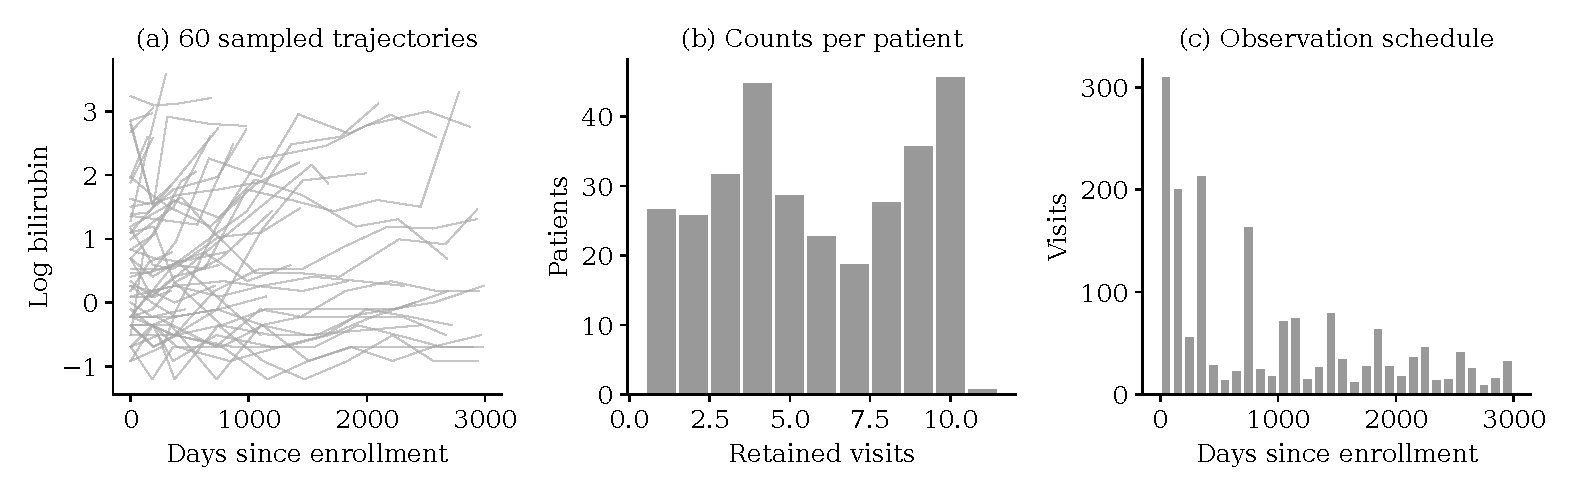
\includegraphics[width=\linewidth]{results/realdata/pbc_data_illustration.pdf}
\caption{PBC trajectories for 60 patients selected with a fixed seed, retained counts, and visit times up to day 3,000. Baseline and scheduled visits are visible.}
\label{fig:pbc-data-new}
\end{figure}

For the separate intercept-only analysis in Figure~\ref{fig:pbc-mean-new}, positive observed bilirubin and the 3,000-day restriction leave 1,790 visits from 312 patients. The equal-subject local linear estimate uses $h=0.09446$, 9,999 multipliers, and the same 201-point evaluation grid as the regression. The critical value is 2.787 and average band width is 0.555. The fit describes the weighted observed visits under the working model. Table~\ref{tab:pbc-new} summarizes the regression bandwidth sensitivity results.
\begin{figure}[!tbp]
\centering
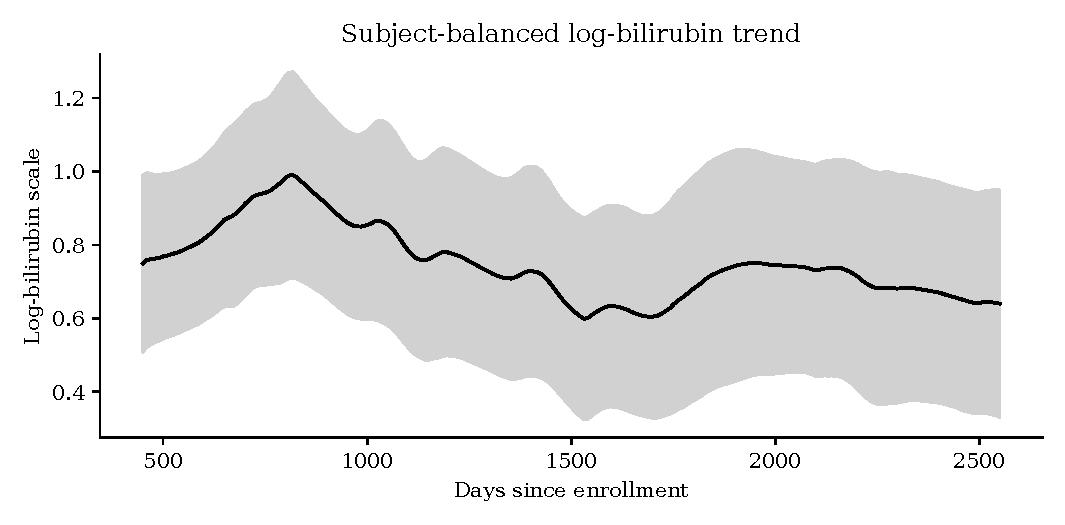
\includegraphics[width=.95\linewidth]{results/realdata/pbc_mean_bands.pdf}
\caption{Subject-balanced log-bilirubin trend and nominal 95\% band under the working sampling model.}
\label{fig:pbc-mean-new}
\end{figure}
\begin{table}[!tbp]
\centering
\caption{PBC nominal joint-band average widths for three bandwidth factors. The primary factor is $c=1$.}\label{tab:pbc-new}
\begin{tabular}{lrrr}
\toprule
Coefficient & $c=0.8$ & $c=1$ & $c=1.2$\\
\midrule
Intercept & 0.774 & 0.647 & 0.602\\
D-penicillamine & 1.056 & 0.899 & 0.846\\
Edema & 0.593 & 0.483 & 0.441\\
Albumin & 0.731 & 0.621 & 0.579\\
Prothrombin time & 0.767 & 0.670 & 0.629\\
Log ALP & 0.579 & 0.500 & 0.467\\
\bottomrule\end{tabular}\end{table}

\FloatBarrier


\referencefont
\referencefont
\bibliographystyle{Chicago}
\bibliography{bibfile}
\end{document}